%
% Template for OPTCON course projects
%
\documentclass[a4paper,11pt,oneside]{book}
\usepackage[latin1]{inputenc}
\usepackage[english]{babel}
\usepackage{amsfonts}
\usepackage{amsmath}
\usepackage{amssymb,amsmath,color}
\usepackage{cite}
\usepackage{graphicx}
\usepackage{float}
\usepackage{subcaption}
\usepackage{geometry}
\usepackage{float}

\geometry{a4paper, margin = 2.5 cm}
\setlength{\parindent}{0pt}
\setlength{\parskip}{10pt}

\begin{document}
\pagestyle{myheadings}

%%%%%%%%%%% Cover %%%%%%%%%%%
\thispagestyle{empty}                                                 
\begin{center}                                                            
    \vspace{5mm}
    {\LARGE UNIVERSIT\`A DI BOLOGNA} \\                       
      \vspace{5mm}
\end{center}
\begin{center}
  
\includegraphics[scale=.27]{figs/logo_unibo}
\end{center}
\begin{center}
      \vspace{5mm}
      {\LARGE School of Engineering} \\
        \vspace{3mm}
      {\Large Master Degree in Automation Engineering} \\
      \vspace{20mm}
      {\LARGE Optimal Control} \\
      \vspace{5mm}{\Large\textbf{Optimal Control of a Flexible Robotic Arm}}                  
      \vspace{15mm}
\end{center}
\begin{flushleft}                                                                              
     {\large Professor: \textbf{\@ Giuseppe Notarstefano}} \\        
      \vspace{13mm}
\end{flushleft}
\begin{flushright}
      {\large Students:\\
      \textbf{Matteo Bonucci\\
      Filippo Samor\`{i}\\
      Jacopo Subini}
      }\\
\end{flushright}        %capoverso allineato a destra
\begin{center}
\vfill
      {\large Academic year \@2024/2025} \\
\end{center}

\newpage
\thispagestyle{empty}

%%%%%%%%%%% Abstract %%%%%%%%%%%%
\begin{center}
\chapter*{}
\thispagestyle{empty}
{\Huge \textbf{Abstract}}\\
\vspace{15mm}
This report presents the development and implementation of the project for the Optimal Control Course at the University of Bologna. The assignment aims to control an underactuated 2-DOF robot manipulator. The report is structured such that each chapter is dedicated to the solution of a specific task.

The project demonstrates the capabilities of the Optimal Control framework in controlling complex systems, such as underactuated systems or time-variant linear systems, such as the linearization of the manipulator system.

The results highlight the robustness in the presence of noise and the variety of possible approaches to the problem.

\end{center}


\tableofcontents \thispagestyle{empty}
% \listoffigures\thispagestyle{empty}

%%%%%%%%%% Introduction %%%%%%%%%%
\chapter*{Introduction}

In this project, we are tasked with designing an optimal trajectory for a flexible robotic arm. Such systems can represent robotic arms used in medical assistance or other precision applications, where flexibility must be taken into account. The flexible arm is simplified and modeled as a planar two-link robot with torque applied to the first joint.

\begin{figure}[H]
    \centering
    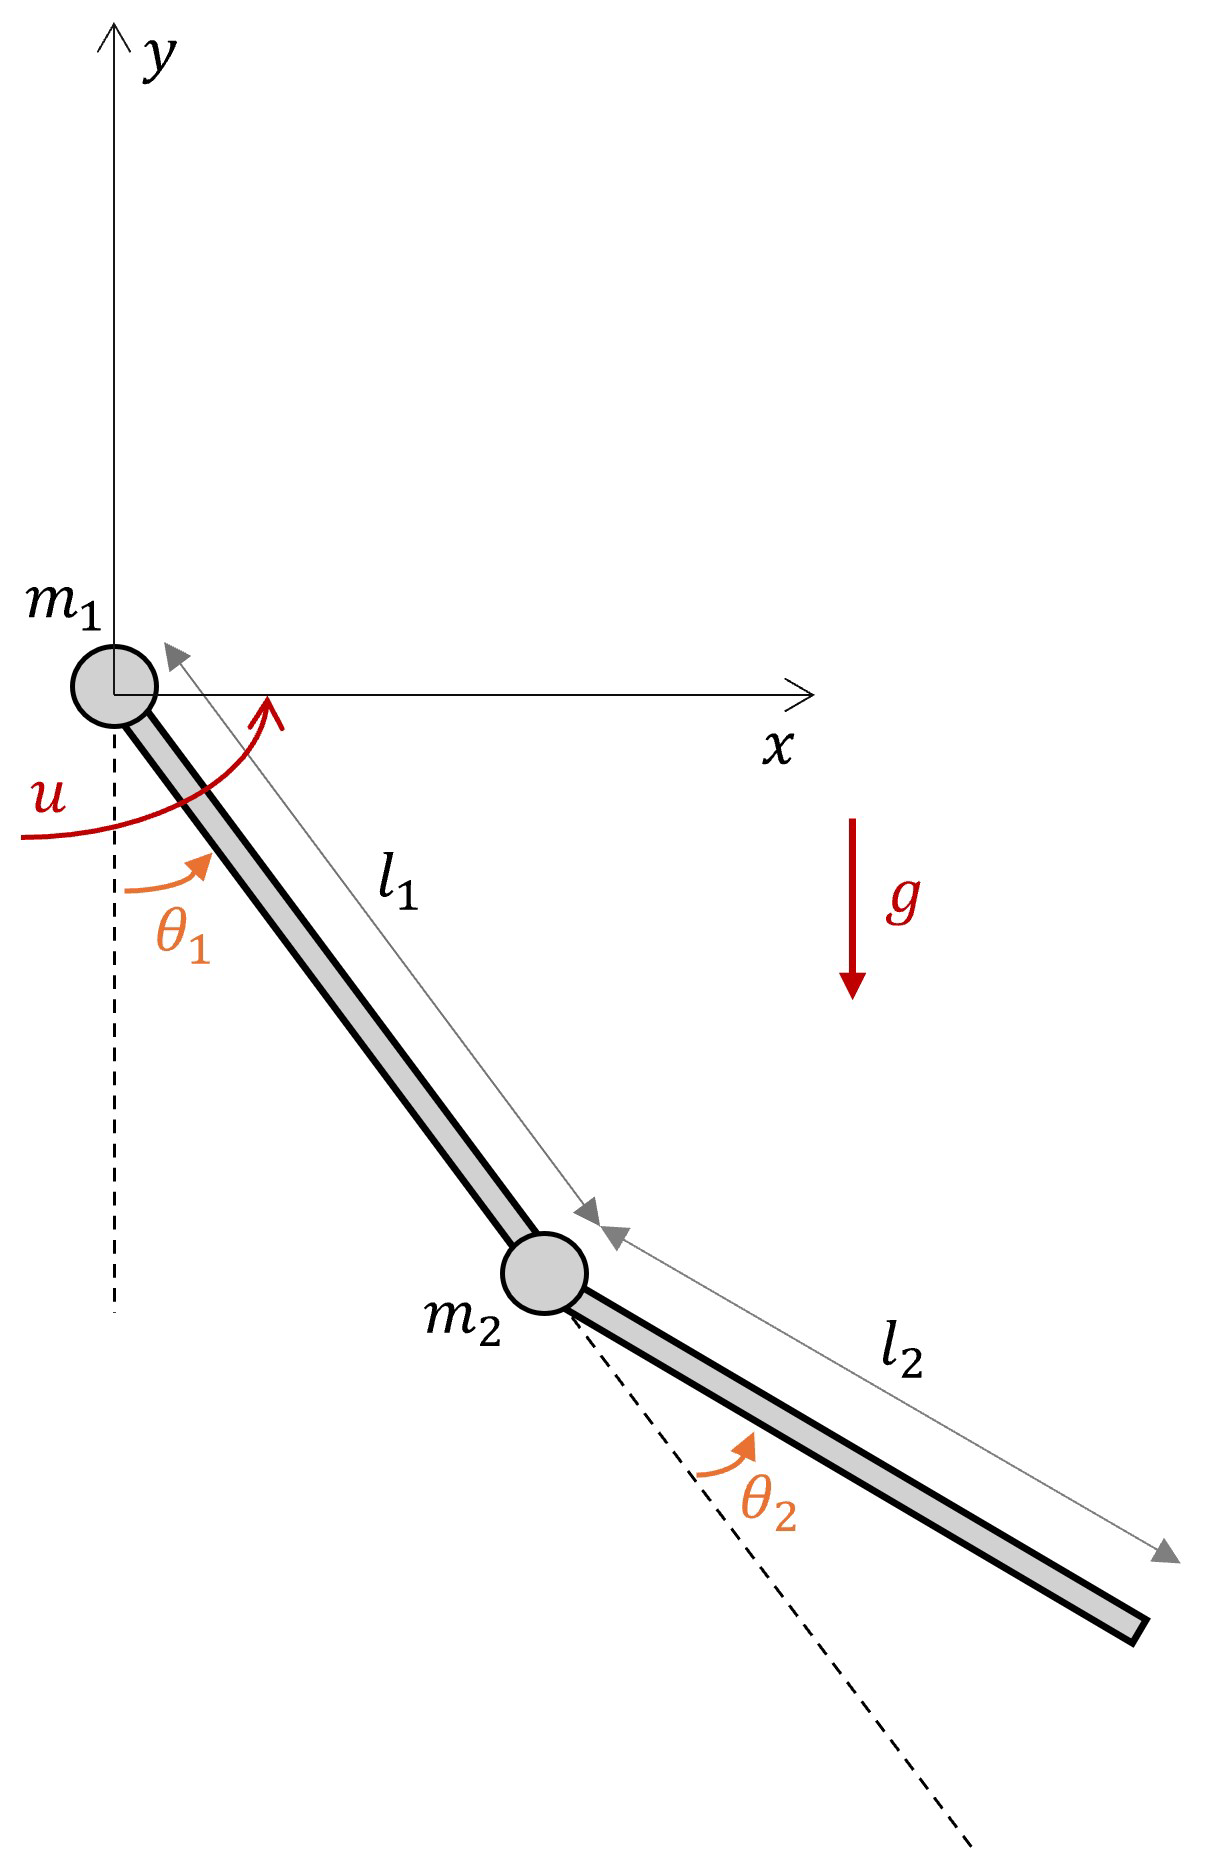
\includegraphics[width=0.35\linewidth]{image.png}
    \caption{2-dof manipulator}
    \label{fig:-2-dof manipulator}
\end{figure}

The 2-dof manipulator dynamics is reported in matrix form: 

\begin{equation}\label{robot dynamics}
    M(q)\Ddot{q} + C(q,\Dot{q}) + G(q) + F\Dot{q} = \begin{bmatrix}
        u \\ 0
    \end{bmatrix}
\end{equation}

The configuration variable $q$ is composed of the angles $\theta_1$ and $\theta_2$, which are defined as the relative angular displacement between the two links.

\begin{equation*}
    \begin{aligned}
    &M = \begin{pmatrix}
        I_1 + I_2 + m_1r_1^2 + m_2(l_1^2 + r_2^2) + 2m_2l_1r_2cos(\theta_2) & I_2 + m_2r_2^2 + m_2l_1r_2cos(\theta_2) \\
        I_2 + m_2r_2^2 + m_2l_1r_2cos(\theta_2) & I_2 + m_2r_2^2
    \end{pmatrix}\\
    & C = \begin{pmatrix}
        -m_2l_1r_2\Dot{\theta}_2sin(\theta_2)(\Dot{\theta}_2 + 2\Dot{\theta}_1) \\
        m_2l_1r_2sin(\theta_2)\Dot{\theta}_1
    \end{pmatrix}\\
    & G = \begin{pmatrix}
       g(m_1r_1 + m_2l_1)sin(\theta_1) + gm_2r_2sin(\theta_1 + \theta_2) \\
       gm_2r_2sin(\theta_1 + \theta_2)
    \end{pmatrix}\\
    & F = \begin{pmatrix}
        f_1 & 0 \\ 0 & f_2
    \end{pmatrix}
    \end{aligned}
\end{equation*}


The parameters of the robot dynamics are described in the table below:

\begin{center}
    \textbf{Parameters : set 1}\\
    \vspace{0.2cm}
    \begin{tabular}{c|c}
    \hline
    $m_1$ & 1 \\
    $m_2$ & 1 \\
    $l_1$ & 1 \\
    $l_2$ & 1 \\
    $r_1$ & 0.5 \\
    $r_2$ & 0.5 \\
    $I_1$ & 0.33 \\
    $I_1$ & 0.33 \\
    $g$ & 9.81 \\
    $f_1$ & 0.1 \\
    $f_2$ & 0.1 
\end{tabular}
\end{center}
 
Task 0: requires writing the dynamics and obtaining the linearization of the system.

Task 1: requires defining a reference transition curve between equilibrium configurations and computing an optimal trajectory between them.

Task 2: requires defining a smooth reference curve between equilibrium configurations and computing again an optimal trajectory. It is suggested to first try tracking the reference with an LQR controller to obtain a feasible initial guess.

Task 3: requires tracking the obtained optimal trajectory with an LQR in the presence of noise.

Task 4: requires tracking the optimal trajectory obtained with an MPC solution in the presence of noise.

Task 5: requires animations for all of the previous tasks.


\addcontentsline{toc}{chapter}{Introduction}

%%%%%%%%%% Chapter Title %%%%%%%%%%

\chapter*{Task 0}
\addcontentsline{toc}{chapter}{Task 0}

Task 0 asks to discretize the dynamics, write the discrete-time state-space equations, and code the dynamics function \texttt{Dynamic.py}.

The state representation is obtained from the formula (\ref{robot dynamics}), defining a state vector $x = [\theta_1 \hspace{0.2cm} \theta_2 \hspace{0.2cm}\Dot{\theta_1} \hspace{0.2cm}\Dot{\theta_2} ]^T$ and writing the dynamics as follows:

\begin{equation}
    \Dot{x} = f(x,u) = \begin{bmatrix}
        x_3 \\
        x_4 \\
        M^{-1}( -G(x_1,x_2) -C(x_1,x_2,x_3,x_4) - F\begin{bmatrix}
            x_3\\x_4
        \end{bmatrix} + \begin{bmatrix}
            u \\ 0
        \end{bmatrix}
    \end{bmatrix}
\end{equation}

The simulations are made numerically by approximating the continuous dynamics with a discrete one using Euler's method for numerical integration. We denote the discrete time state vector as $x_t$, where the subscript describes the discrete time instant.

\begin{equation}\label{Discretized traj}
    x_{t+1} = x_t + \Dot{x}\Delta t = x_t + f(x_t,u_t)\Delta t = f_{dis}(x_t,u_t)
\end{equation}

The linearization matrices are obtained by computing the Jacobian of $f_d(x_t,u_t)$ with respect to $x_t$ for matrix $A_t$ and $u_t$ for matrix $B_t$. They are time-varying if the linearization is computed about a trajectory of the system.

It is possible to compute the discrete matrices starting from the continuous-time Jacobians and obtaining $A_t$ and $B_t$ by discretizing.


\begin{equation} \label{con_to_dis}
        \Delta x_{t+1} = (I_{n\times n} + \frac{\partial f}{\partial x}\bigg|_{x_t,u_t} \Delta t) \Delta x_t + 
        (\frac{\partial f}{\partial u}\bigg|_{x_t,u_t} \Delta t) \Delta u_t
\end{equation}

\begin{equation*}
    A_t = I_{n\times n} + \frac{\partial f}{\partial x}\bigg|_{x_t,u_t} \Delta t = \nabla_1f_{dis}(x,u)^T
\end{equation*}

\begin{equation*}
    B_t = \frac{\partial f}{\partial u}\bigg|_{x_t,u_t} \Delta t = \nabla_2f_{dis}(x,u)^T
\end{equation*}

To compute the derivatives, the symbolic Python package SymPy has been used. The package computes the continuous dynamic Jacobians directly, and then we obtain the discrete Jacobians using (\ref{con_to_dis}).

\section*{Python code}

The discrete dynamics are implemented in Python in the file \texttt{Dynamics.py}. In the code, four main functions are defined:

\begin{itemize}
    \item \textbf{gravity(xx) }: compute the gravity torque applied to the motor in joint one at a specific state x.\\\\
    \textbf{Arguments}:
    \begin{itemize}
        \item xx : state vector.
    \end{itemize}
    \textbf{Return}:
    \begin{itemize}
        \item gravity : torque value.
    \end{itemize}

    \item \textbf{dynamics(xx,uu,dt) }: Compute the future state $x_{t+1}$ given the states $x_t$ and the input $u_t$. The functions first compute the continuous dynamics $f(x,u)$ of the manipulator (\ref{robot dynamics}) and then discretize it using (\ref{Discretized traj}). \\\\
    \textbf{Arguments}:
    \begin{itemize}
        \item xx : state vector at time t.
        \item uu : input vector at time t.
        \item dt : time of dicretization.
    \end{itemize}
    \textbf{Return}:
    \begin{itemize}
        \item xx\_plus : computed state at time t+1. 
    \end{itemize}

    \item \textbf{linearized\_dynamics\_symbolic()}: Compute the symbolic Jacobians of the continuous dynamics with respect to $x$ and $u$. The computations are made using the Python package Sympy. The symbolic terms are computed only once and then used by other functions to compute the numerical values by substitution of values.
  \\\\
    \textbf{Arguments}:
    \begin{itemize}
        \item None.
    \end{itemize}
    \textbf{Return}:
    \begin{itemize}
        \item A\_func : Symbolic jacobian respect to x.
        \item B\_func : Symbolic jacobian respect to u.
    \end{itemize}

    \item \textbf{linearized\_dynamics\_numeric(xx,uu,A\_func,B\_func,dt)}: Compute the numerical value of the Jacobians of the discrete dynamics with respect to $x$ and $u$. The computations are made using the continuous symbolic Jacobians computed from \texttt{linearized\_dynamics\_symbolic()} and then applying the formulas from (\ref{con_to_dis}) to compute the discrete ones. \\\\
    \textbf{Arguments}:
    \begin{itemize}
        \item xx : state vector at time t.
        \item uu : input vector at time t.
        \item A\_func : Symbolic jacobian respect to x.
        \item B\_func : Symbolic jacobian respect to u.
        \item dt : time of dicretization.
    \end{itemize}
    \textbf{Return}:
    \begin{itemize}
        \item A\_dis : Numeric jacobian respect to x at time t.
        \item B\_dis : Numeric jacobian respect to u at time t.
    \end{itemize}
\end{itemize}

\chapter*{Task 1}
\addcontentsline{toc}{chapter}{Task 1}

Task 1 requires computing two equilibrium points for the system, defining a reference curve between them. Then, it is required to compute an optimal trajectory to move from one equilibrium to another using the Newton's-like algorithm.

In general, the equilibrium points are all the points that satisfy the equation:

\begin{equation}
    x_{e} = f_{dis}(x_e,u_e)
\end{equation}

In our case, the discrete dynamics are the one described in (\ref{Discretized traj}), so a condition for equilibrium becomes that:

\begin{equation}
    x_e = x_e + f(x_e,u_e)\Delta t \longrightarrow f(x_e,u_e) = 0
\end{equation}

That means that the equilibrium points for the discrete dynamics are equal to those of the continuous dynamics.

Since the second joint is not controlled, the system is in equilibrium only if the second joint is in equilibrium. As we know for a simple pendulum, the equilibrium configurations are the ones where the absolute angle $\theta$ with respect to the world frame is equal to 0 or $\pi$. The world frame is defined such that the $y$ axis is parallel to the gravity vector and it is equal to the frame of joint one. So, we have that the second link is in equilibrium for each value of $q_2$ such that $q_1 + q_2 = 0 \text{ or } \pi$.

So, for the whole system, we have equilibrium when the velocities are zero, the input compensates for the gravity in the first joint (\ref{eq input}), and the second joint satisfies the equation $q_1 + q_2 = 0 \text{ or } \pi$.

\begin{equation} \label{eq input}
    u = G_1(q)
\end{equation}

Once two equilibrium points have been chosen, it is necessary to run the Newton's-like method with an initial guess that is a valid trajectory of the system. For our purposes, in task 1, we initialize the initial guess as constant vectors in the chosen initial equilibrium configuration.

The cost function is defined as follows:

\begin{equation}\label{Cost function}
\begin{aligned}
        \ell(x,u) = \sum_{t=0}^{T-1} (x_t - x_t^{ref})^TQ_t(x_t - x_t^{ref}) + (u_t-u_t^{ref})^TR_t(u_t-u_t^{ref})\\
        + (x_T - x_T^{ref})^TQ_T(x_T - x_T^{ref})
\end{aligned}
\end{equation}

and the unconstrained optimal control problem is stated as:

\begin{equation}
    \begin{aligned}
        &\min_{x \hspace{0.1cm}u} \hspace{0.1cm}\ell(x,u) \\
        &subj. to \hspace{0.5cm} x_{t+1} - f_d(x_t,u_t) = 0
    \end{aligned}
\end{equation}

The cost is a quadratic function of the states and the inputs. The Newton's-like method solves at each iteration a convex quadratic approximation of the whole problem, computing the descent direction as the solution of the Linear Quadratic Regulator.

The optimization is solved by considering an augmented state vector with the corresponding augmented matrices.

\begin{equation*}
    \Delta\Tilde{x}_t := \begin{bmatrix}
        1 \\
        \Delta x_t\end{bmatrix} 
\end{equation*}

\begin{equation*}
        q_t = \nabla_1 \ell(x_t^k,u_t^k) = Q_t(x_t^k - x_t^{ref}) \quad r_t = \nabla_2 \ell(x_t^k,u_t^k) = R_t(u_t^k - u_t^{ref})
\end{equation*}
            
\begin{equation*}
    Q_t = \nabla_{11} \ell(x_t^k,u_t^k) \quad R_t = \nabla_{22} \ell(x_t^k,u_t^k)
\end{equation*}

\begin{equation*}
    \Tilde{Q}_t := \begin{bmatrix}
        0 & q_t^T\\
        q_t & Q_t
    \end{bmatrix} \hspace{0.3cm}
    \Tilde{S}_t := \begin{bmatrix}
        r_t & S_t
    \end{bmatrix} \hspace{0.3cm}
    \Tilde{R}_t := R_t \hspace{0.3cm}
    \Tilde{A}_t := \begin{bmatrix}
        1 & 0\\
        c_t & A_t
    \end{bmatrix} \hspace{0.3cm}
    \Tilde{B}_t := \begin{bmatrix}
        0\\
        B_t
    \end{bmatrix} \hspace{0.3cm}
\end{equation*}

Then the associated LQR problem can be solved using the Difference Riccati Equation (\ref{Diff ricc eq}) for the matrix $P$ and computing the optimal gain $\Tilde{K}^*$ \footnote{The * denotes an optimal result}. To solve the problem, we use a regularized Newton's-like method where the terms $\nabla_{11}f_d(x_t^k,u_t^k)$ and $\nabla_{22}f_d(x_t^k,u_t^k)$ are ignored. In this way, we are sure that the matrices $\Tilde{Q}_t$ and $\Tilde{R}_t$ are always positive (semi-\footnote{The matrix $Q_t$ must be semi-positive definite, the matrix $R_t$ must be positive definite}) definite.

\begin{equation}
    \begin{aligned}
    &\min_{\Delta x \Delta u} \sum_{t=0}^{T-1} 
    \frac{1}{2}\begin{bmatrix}
        \Delta\Tilde{x}_t \\
        \Delta u_t
    \end{bmatrix}^T
    \begin{bmatrix}
        \Tilde{Q}_t & \Tilde{S}_t^T\\
        \Tilde{S}_t & \Tilde{R}_t
    \end{bmatrix}
    \begin{bmatrix}
        \Delta\Tilde{x}_t \\
        \Delta u_t
    \end{bmatrix}+\frac{1}{2} \Delta\Tilde{x}_T^T\Tilde{Q}_T\Delta\Tilde{x}_T \\
    & s.t. \hspace{0.5cm} \Delta\Tilde{x}_{t+1} = \Tilde{A}_t\Delta\Tilde{x}_t + \Tilde{B}_t\Delta\Tilde{u}_t \quad t = 0,..,T-1
    \end{aligned}
\end{equation}

The Difference Riccati Equation (\ref{Diff ricc eq}) is solved by backward integration, with the initial condition $P_T = \Tilde{Q}_T$.

\begin{equation}
    \Tilde{K}_t^* = -(\Tilde{R}_t + \Tilde{B}_t^T P_{t+1} \Tilde{B}_t)^{-1}(\Tilde{S}_t + \Tilde{B}_t^T P_{t+1} \Tilde{A}_t)
\end{equation}

\begin{equation} \label{Diff ricc eq}
    P_t = \Tilde{Q}_t + \Tilde{A}_t^T P_{t+1} \Tilde{A}_t - K_t^{*T}(\Tilde{R}_t + \Tilde{B}_t^T P_{t+1} \Tilde{B}_t )K_t^* \quad t = T-1,...,0
\end{equation}

To solve the convex quadratic problem, a shooting approach is considered. The solution is computed for $\Delta u$, and then $\Delta x$ is obtained through forward integration of the linearized dynamics.

\begin{equation}
    \begin{aligned}
        &\Delta\Tilde{u}_t = \Tilde{K}_t^*\Delta\Tilde{x}_t\\
        &\Delta\Tilde{x}_{t+1} = \Tilde{A}_t\Delta\Tilde{x}_t + \Tilde{B}_t\Delta\Tilde{u}_t
    \end{aligned}
\end{equation}

Once the descent direction $\Delta u^k$ is computed, the global solution can be updated using a robustified feedback integration of the dynamics. The step size can be chosen fixed or computed using Armijo's rule. Armijo's method is also useful to understand if the actual solution $\Delta u^k$ is effectively a descent direction, and it helps to check if the linearization of the dynamics is correctly computed by checking if the line (\ref{red line}), parametrized by $\gamma$, is tangent to the current cost $\ell(x^k,u^k)$.

\begin{equation} \label{red line}
    y(\gamma) = J(u^k) + \gamma \nabla J(u^k)^T\Delta u^k
\end{equation}

The step size selection condition for Armijo's rule is

\begin{equation}
    J(u^k + \gamma\Delta u^k) \geq J(u^k) + \gamma \nabla J(u^k)^T\Delta u^k
\end{equation}

\begin{equation}
    \begin{aligned}
        &u_t^{k+1} = u_t^{k} + K_t^k(x_t^{k+1}-x_t^k) + \gamma^k\sigma_t^k\\
        & x_{t+1}^{k+1} = f_d(x_t^{k+1},u_t^{k+1})        
    \end{aligned}
\end{equation}

The algorithm stops the iterations when it finds a descent direction whose squared amplitude is lower than a certain threshold, or when Armijo's method fails to determine a feasible step size.

In our case, we have chosen the following equilibrium point:

\begin{equation*}
\begin{aligned}
    &x_{init} = [0,0,0,0] \\
    &x_{fin} = [90,-90,0,0]
\end{aligned}  
\end{equation*}

These points are easy to reach because they are stable. A step reference transition has been chosen (Fig \ref{fig:downward_0}). The simulation time is set to 10 seconds, and the discretization time is 0.01 seconds. 

The weights in the cost have been selected experimentally, and a good compromise resulted in:

\begin{equation*}
    \begin{aligned}
        &Q_t = \begin{bmatrix}
            1000 & 0 & 0 & 0 \\
            0 & 1000 & 0 & 0 \\
            0 & 0 & 10 & 0\\
            0 & 0 & 0 & 10
        \end{bmatrix} = Q_T\\
        &\\
    & R_t = 10
    \end{aligned}
\end{equation*}

The algorithm requires 8 iterations to converge to a solution. As shown in the descent direction figure (\ref{fig:Downward_Descent}), the value of the norm falls below $10^{-6}$, which is the value chosen for the threshold.

The Armijo parameters have been selected using the values from the course slides:

\begin{itemize}
    \item $\beta$ = 0.7
    \item  $c$ = 0.5
\end{itemize}

\begin{figure}
    \centering
    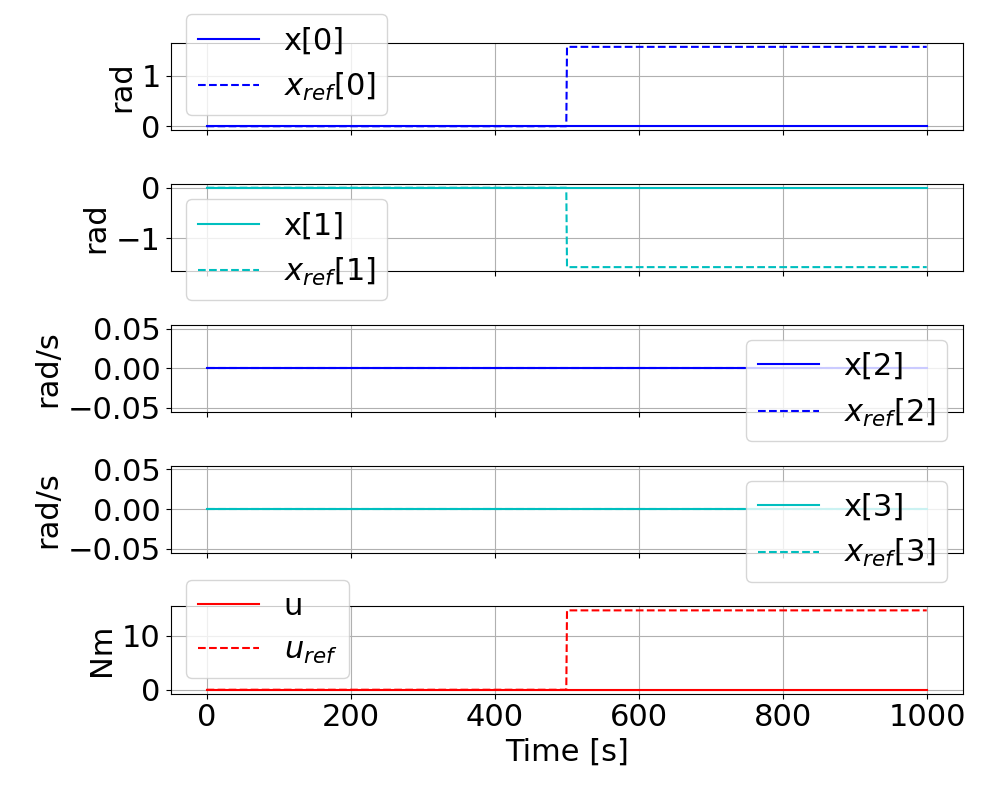
\includegraphics[width=0.8\linewidth]{figs/downwards_0.png}
    \caption{Reference and initial guess}
    \label{fig:downward_0}
\end{figure}

\begin{figure}
    \centering
    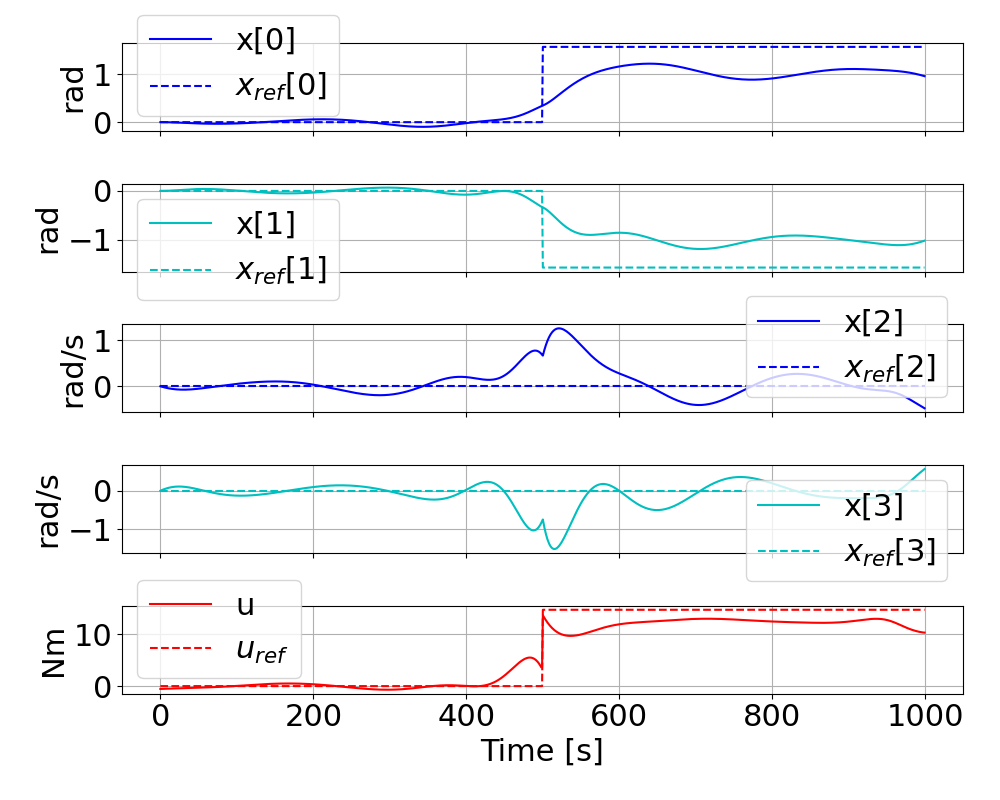
\includegraphics[width=0.8\linewidth]{figs/downwards_1.png}
    \caption{First iteration}
    \label{fig:downwards_1}
\end{figure}

\begin{figure}
    \centering
    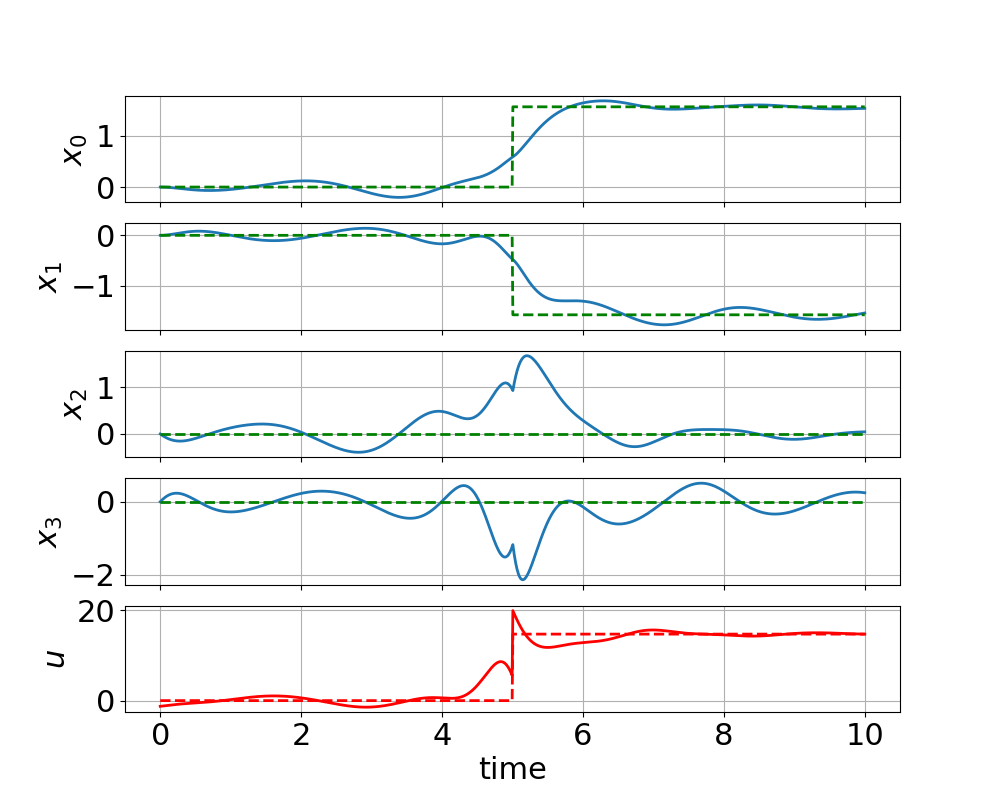
\includegraphics[width=0.8\linewidth]{figs/downwards_f.png}
    \caption{Final result}
    \label{fig:downward_f}
\end{figure}

\begin{figure}
    \centering
    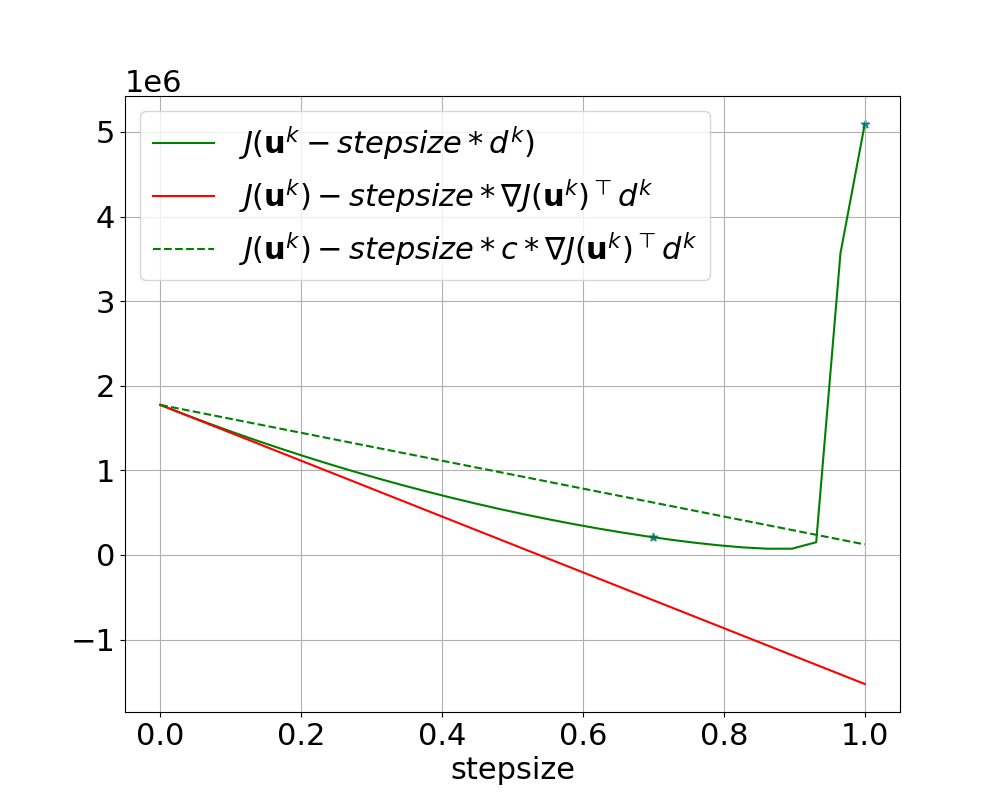
\includegraphics[width=0.8\linewidth]{figs/downward_armijio_0.png}
    \caption{Backtracking line search plot at the first iteration}
    \label{fig:downward_armijio_0}
\end{figure}

\begin{figure}
    \centering
    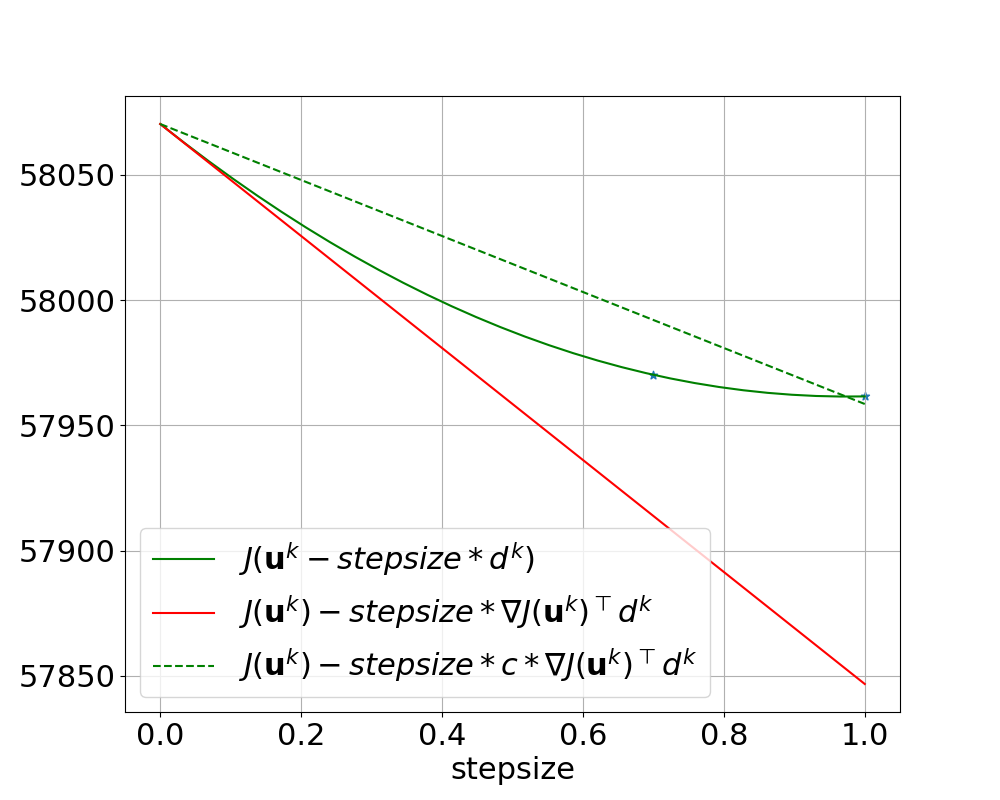
\includegraphics[width=0.8\linewidth]{figs/downward_armijio_3.png}
    \caption{Backtracking line search plot at the third iteration}
    \label{fig:downward_armijio_3}
\end{figure}

\begin{figure}
    \centering
    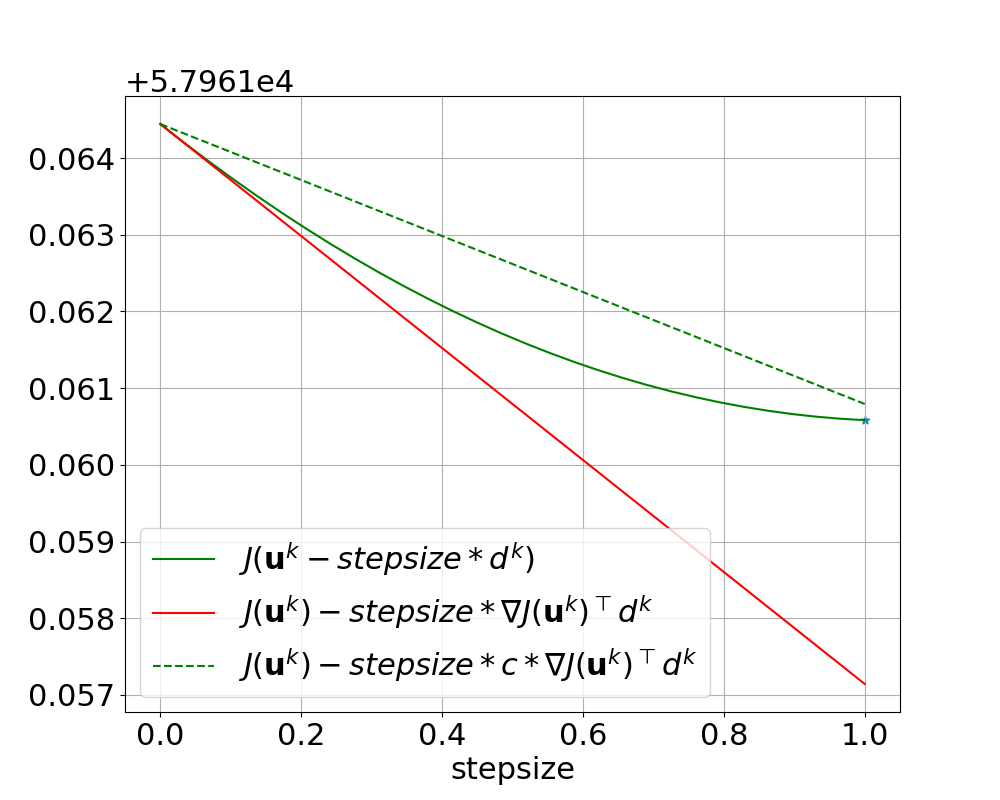
\includegraphics[width=0.8\linewidth]{figs/downward_armijio_6.png}
    \caption{Backtracking line search plot at the sixth iteration}
    \label{fig:downward_armijio_6}
\end{figure}

\begin{figure}[htbp]
    \centering
    \begin{subfigure}[b]{0.49\textwidth}
        \centering
        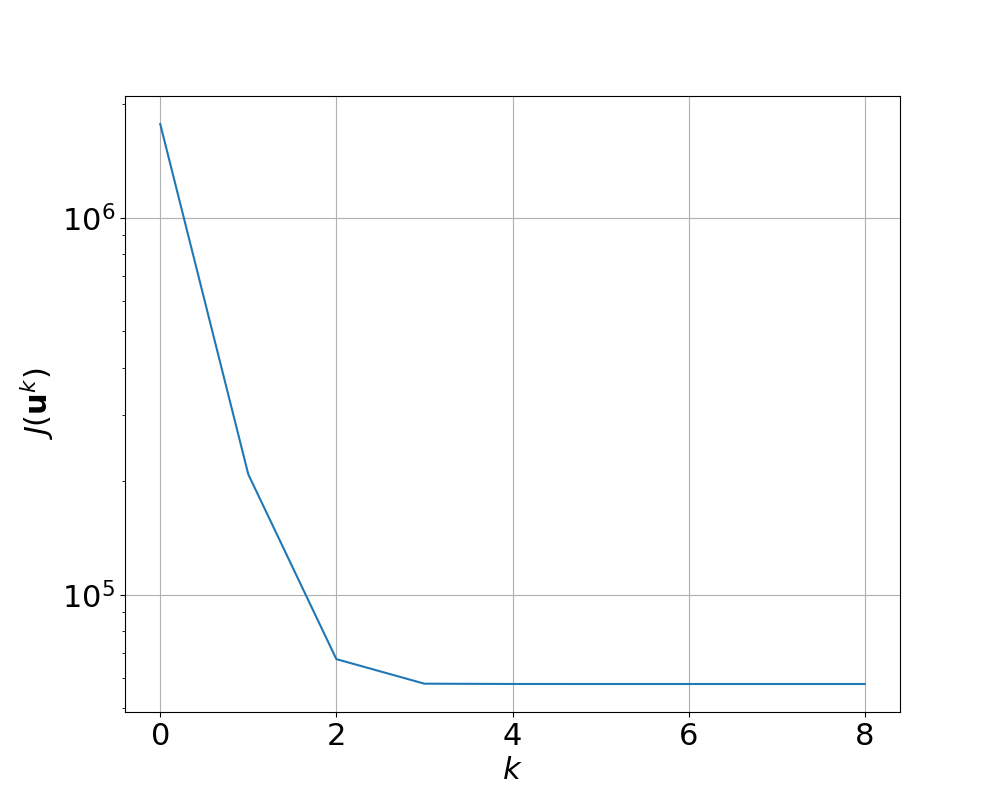
\includegraphics[width=\textwidth]{figs/downward_cost.png}
        \caption{Cost}
        \label{fig:downward_cost}
    \end{subfigure}
    \hfill
    \begin{subfigure}[b]{0.49\textwidth}
        \centering
        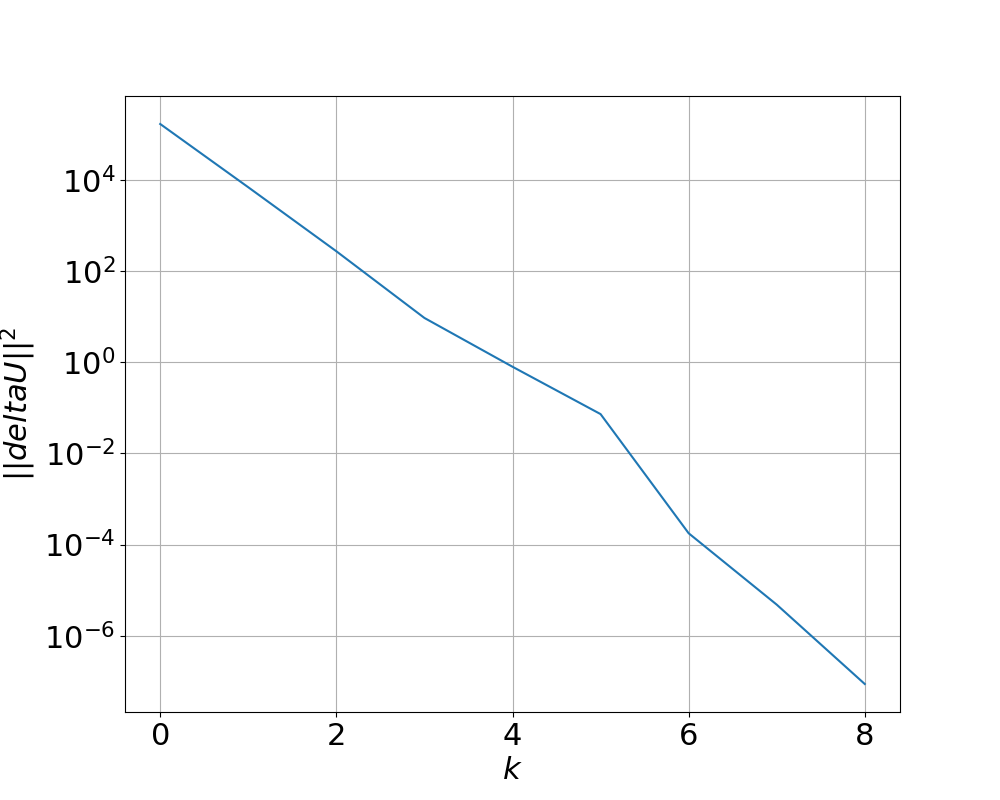
\includegraphics[width=\textwidth]{figs/Downward_Descent.png}
        \caption{Descent direction}
        \label{fig:Downward_Descent}
    \end{subfigure}
    \caption{}
\end{figure}

\section*{Python code}
The reference trajectory is defined in the Python file reference\_trajectory.py.

The Newton's method solver is defined in the Python file solver.py.

\begin{itemize}
    \item \textbf{step(xx\_init, xx\_fin, tf, dt) }Compute a step curve between xx\_init and xx\_fin. The input is calculated as the gravity compensation along the resulting state reference curve.\\\\
    \textbf{Arguments}:
    \begin{itemize}
        \item xx\_init : Initial state vector in degrees.
        \item xx\_fin : Final state vector in degrees.
        \item tf : Final time in seconds.
        \item dt : Time of dicretization in seconds.
    \end{itemize}
    \textbf{Return}:
    \begin{itemize}
        \item xx\_ref : Reference curve between the two states from 0 to tf, in radiants.
        \item uu\_ref : Input reference curve.
    \end{itemize}
    
    \item \textbf{step\_comp(points, tf, dt) }: Compute a composition of step curves between state configuration points. The input is calculated as the gravity compensation along the resulting state reference curve.\\\\
    \textbf{Arguments}:
    \begin{itemize}
        \item points : List of state vectors in degrees.
        \item tf : Final time in seconds.
        \item dt : Time of dicretization in seconds.
    \end{itemize}
    \textbf{Return}:
    \begin{itemize}
        \item xx\_ref : State reference curve in radiants.
        \item uu\_ref : Input reference curve.
    \end{itemize}

\item \textbf{newton\_solver(xx\_ref, uu\_ref, xx\_init, uu\_init, dyn, tf, dt, max\_iters, ...) }: Compute the optimal trajectory using the Newton's-like method. The Armijo's method is also implemented for the selection of the step size. \\\\
    \textbf{Arguments}:
    \begin{itemize}
        \item xx\_ref : Reference state curve.
        \item uu\_ref : Reference input curve.
        \item xx\_init : Initial guess state trajectory.
        \item uu\_init : Initial guess input trajectory.
        \item dyn : dynamic package imported from Dinamics.py.
        \item tf : Final simulation time, in seconds.
        \item dt : Time of dicretization in seconds.
        \item max\_iters : Maximum number of iteration of the algorithm.
        \item term\_cond = 1e-1 : Is the terminal condition for the squared magnitude of the discent direction.
        \item fixed\_stepsize = 1e-1 : Step size value if Armijio is not enabled.
        \item armijo = False : Armijo enable variable.
        \item dynamic\_plot = False : Plot while executing.
        \item visu\_descent\_plot = False : Armijio plot.
        \item armijo\_maxiters = 20 : Maximum number of iteration for the stepsize search.
        \item cc = 0.5 : Armijo paramiter.
        \item beta = 0.7 : rate of reduction of the stepsize at each armijo iteration.
        \item stepsize\_0 = 1 : Initial Armijo stepsize.
    \end{itemize}
    
    \textbf{Return}:
    \begin{itemize}
        \item xx\_star : Optimal State Trajectory.
        \item uu\_star : Optimal Input Trajectory.
        \item JJ : Vector of acquired costs.
        \item descent : Squared value of the magnitude of the descent direction.
        \item max\_iter : Number of effective iterations.
    \end{itemize}

\end{itemize}

\chapter*{Task 2}
\addcontentsline{toc}{chapter}{Task 2}

Task 2 requires computing a smooth state-input curve. Then, it is required to compute the optimal trajectory as in Task 1.

We have designed the trajectory as a smooth transition between equilibrium points.

Since we have to impose the initial and final configurations and velocities for each joint, we need at least a third-order polynomial curve to transit from one equilibrium point to another.

For the first joint $q_1$, we impose the initial and final angles, both with zero velocity. The corresponding curve is defined as:


\begin{equation} \label{smooth_q1}
    \begin{aligned}
         &q_1(t) = a_0 + a_1t + a_2 t^2 + a_3 t^3 \\
         &\Dot{q_1}(t) = a_1 + 2a_2 t + 3a_3 t^2 \\
         &a_0 = q_{1i}\\
         &a_1 = 0\\
         &a_2 = 3 (q_{1f} - q_{1i})/(t_f^2)\\
         &a_3 = -2 (q_{1f} - q_{1i})/(t_f^3)
    \end{aligned}
\end{equation}

For the second joint $q_2$, we compute it as
\begin{equation} \label{smooth_q2}
    \begin{aligned}
            &q_2(t) = z - q_1(t) \quad z = 0 \lor \pi \\
            &\Dot{q}_2(t) = - \Dot{q}_1(t)
    \end{aligned}
\end{equation}

The value of $z$ is chosen depending on the configuration we want to maintain:

\begin{itemize}
    \item $z = \pi$, the second link is pointing upwards.
    \item $z = 0$, the second link is pointing downwards.
\end{itemize}

The input is computed as the gravity compensation along the smooth curve.

Once the reference has been computed, to improve the initial guess used to start the Newton's method algorithm, we try to track the reference with an LQR feedback computed on the linearization about it.

Since the trajectory is a sequence of equilibria, we get a solution for the LQR, only if the motions are quite slow. The reason is that if we try to track a quasi-static trajectory, since the second joint is not actuated, it is difficult for the control law to track the reference for fast motions.

Moreover, since the reference is not a true trajectory, the linearized dynamics is of the form:

\begin{equation}
\begin{aligned}
       &\Delta x_{t+1} = A_t \Delta x_t + B_t \Delta u_t + c_t \\
       & c_t = f(x^{ref}_t,u^{ref}_t) - x^{ref}_{t+1}
\end{aligned}    
\end{equation}

where the $c_t$ term is not zero.

In this case, we have chosen the same equilibrium points as before:

\begin{equation*}
\begin{aligned}
    &x_{init} = [0,0,0,0] \\
    &x_{fin} = [90,-90,0,0]
\end{aligned}  
\end{equation*}

A smooth reference transition has been chosen (Fig \ref{fig:downward_0_smooth}), and as it is possible to see, it is much easier to track than a step. The time of simulation is selected as 10 seconds, and the discretization time is 0.01 seconds.

The weights in the cost have been selected as before:

\begin{equation*}
    \begin{aligned}
        &Q_t = \begin{bmatrix}
            1000 & 0 & 0 & 0 \\
            0 & 1000 & 0 & 0 \\
            0 & 0 & 10 & 0\\
            0 & 0 & 0 & 10
        \end{bmatrix} = Q_T\\
        &\\
    & R_t = 10
    \end{aligned}
\end{equation*}

The algorithm takes 3 iterations to converge to a solution. As can be seen from the descent direction figure (\ref{fig:Downward_Descent_smooth}), the value of the norm goes below $10^{-6}$, which is the value we chose for the threshold.

\begin{figure}
    \centering
    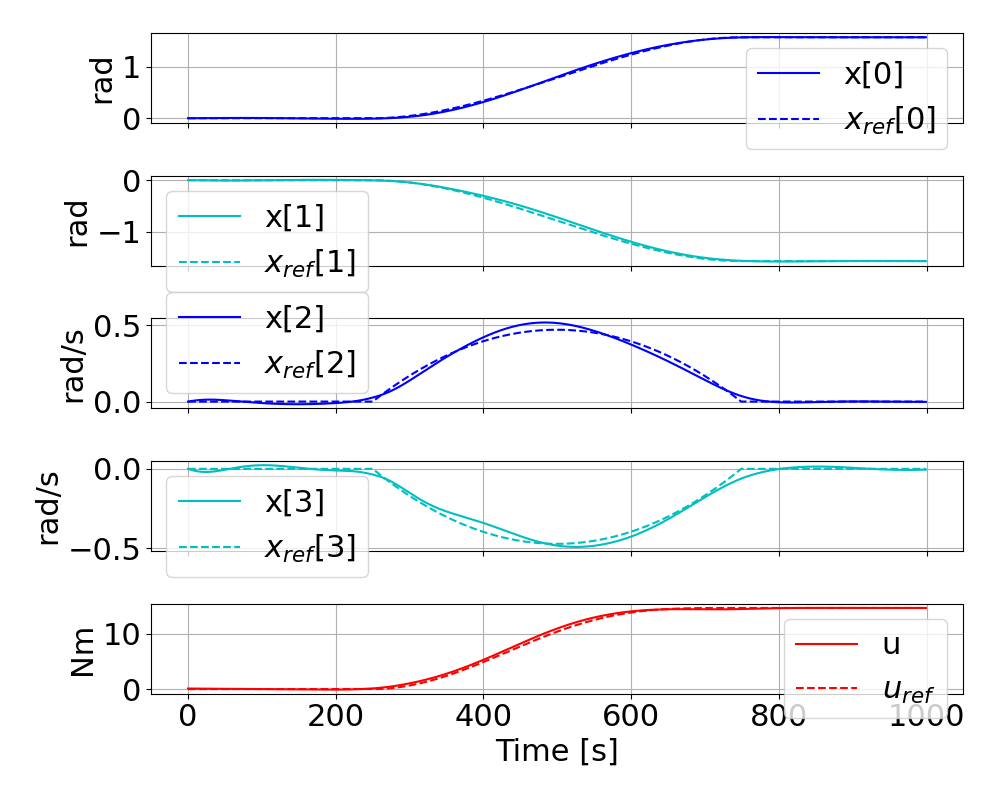
\includegraphics[width=0.8\linewidth]{figs/downward_0_smooth.png}
    \caption{Reference and initial guess}
    \label{fig:downward_0_smooth}
\end{figure}

\begin{figure}
    \centering
    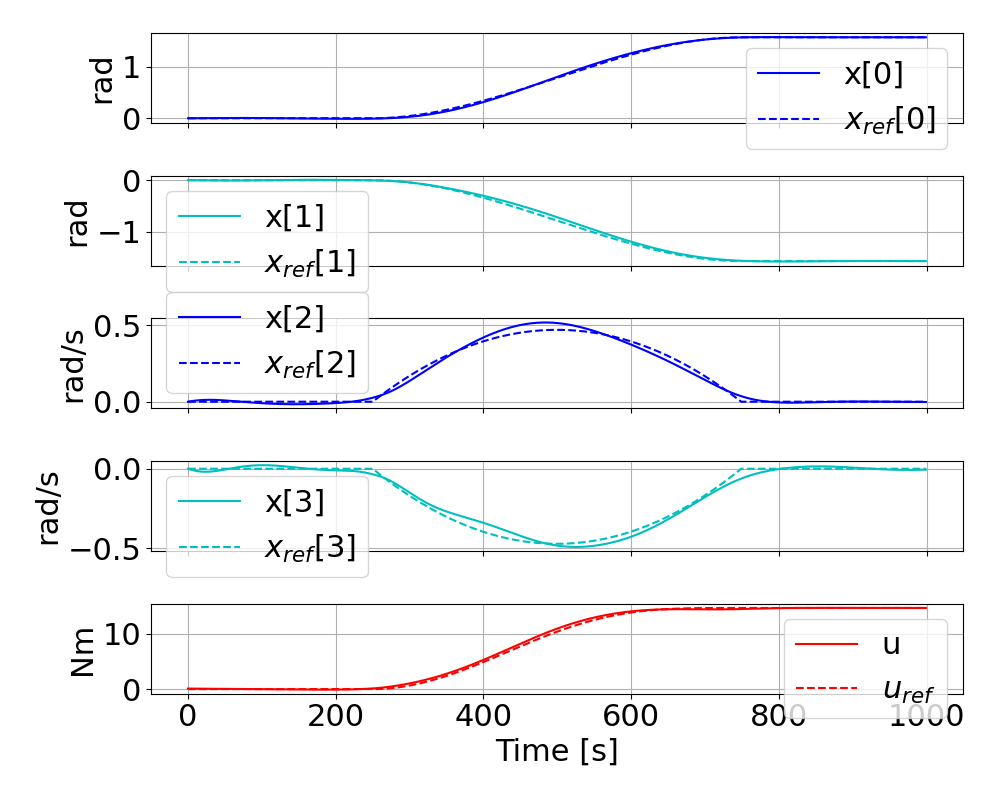
\includegraphics[width=0.8\linewidth]{figs/downward_1_smooth.png}
    \caption{First iteration}
    \label{fig:downward_1_smooth}
\end{figure}

\begin{figure}
    \centering
    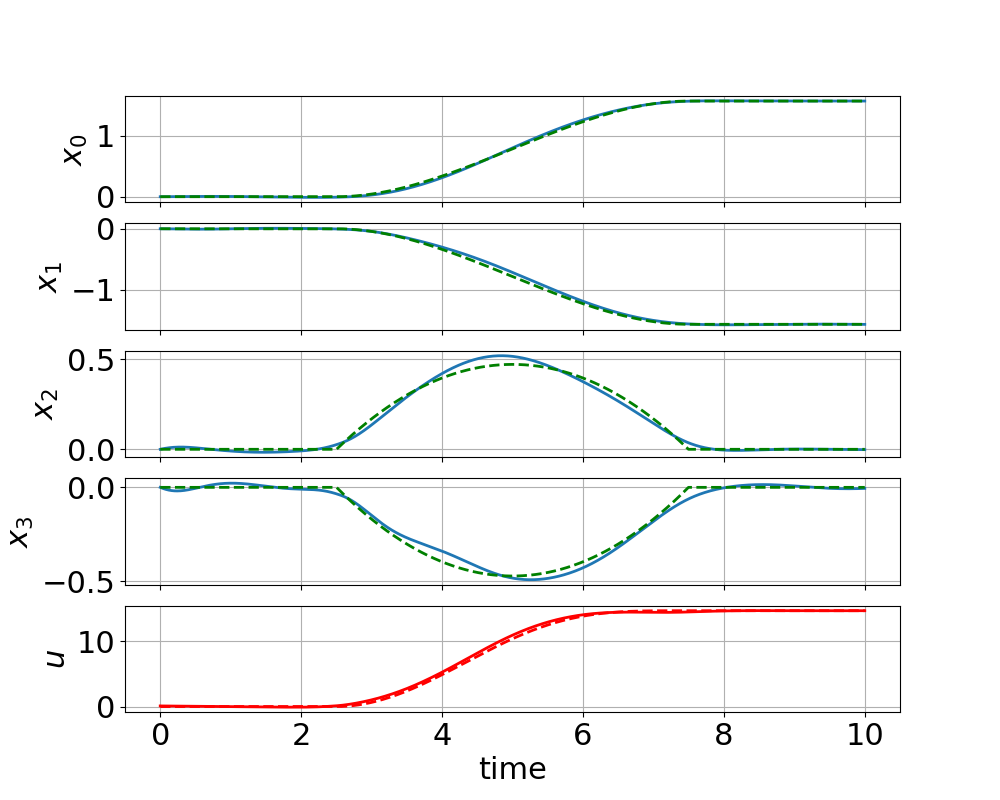
\includegraphics[width=0.8\linewidth]{figs/downward_f_smooth.png}
    \caption{Final result}
    \label{fig:downward_f_smooth}
\end{figure}

\begin{figure}
    \centering
    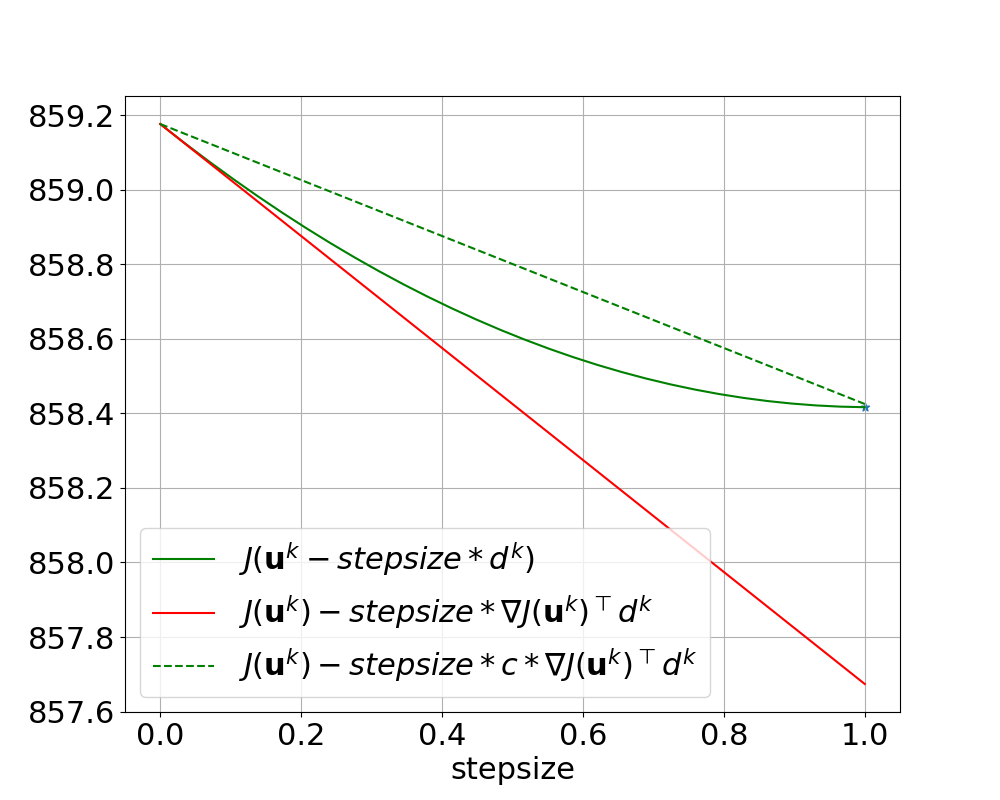
\includegraphics[width=0.8\linewidth]{figs/downward_armijio_0_smooth.png}
    \caption{Backtracking line search plot at the first iteration}
    \label{fig:downward_armijio_0_smooth}
\end{figure}

\begin{figure}
    \centering
    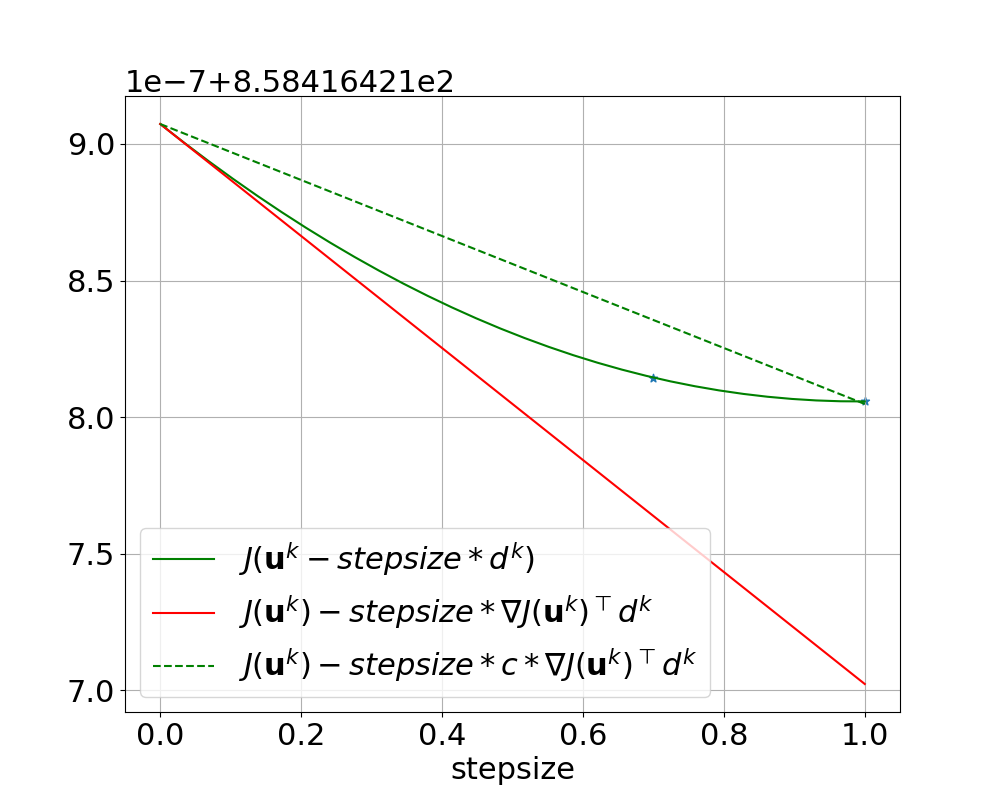
\includegraphics[width=0.8\linewidth]{figs/downward_armijio_f_smooth.png}
    \caption{Backtracking line search plot at the final iteration}
    \label{fig:downward_armijio_f_smooth}
\end{figure}

\begin{figure}
    \centering
    \begin{subfigure}[b]{0.49\textwidth}
        \centering
        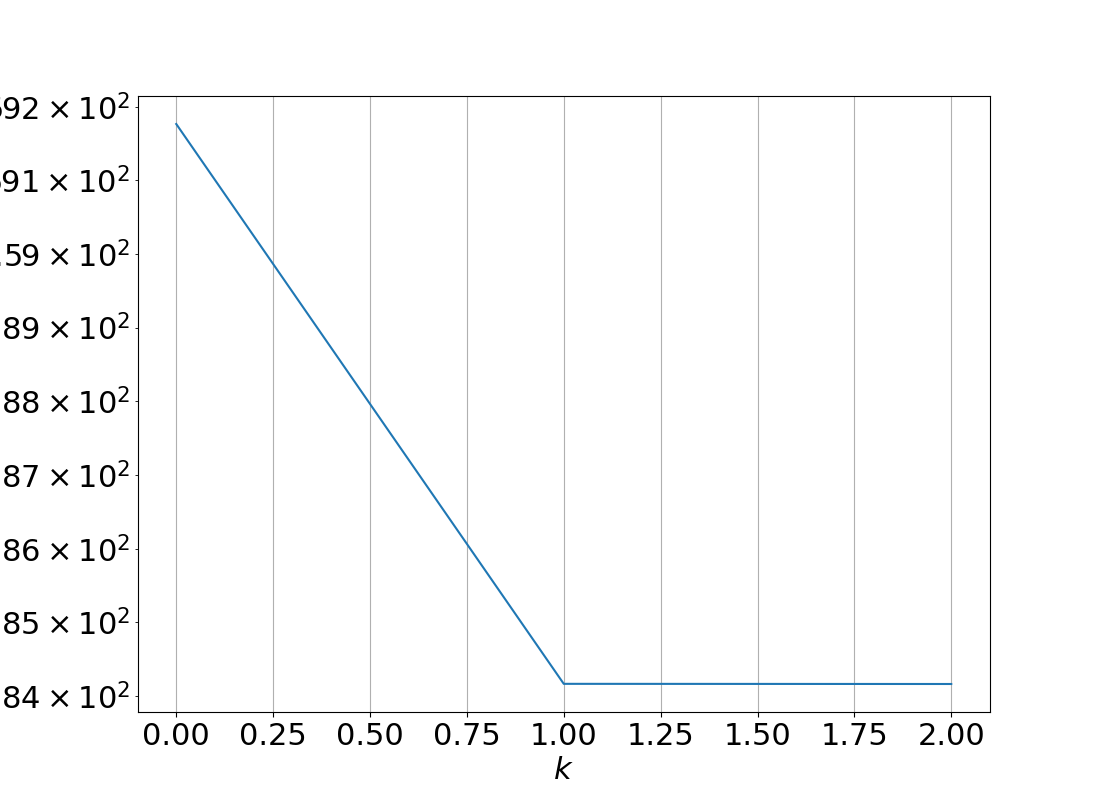
\includegraphics[width=\textwidth]{figs/downward_cost_smooth.png}
        \caption{Cost}
        \label{fig:downward_cost_smooth}
    \end{subfigure}
    \hfill
    \begin{subfigure}[b]{0.49\textwidth}
        \centering
        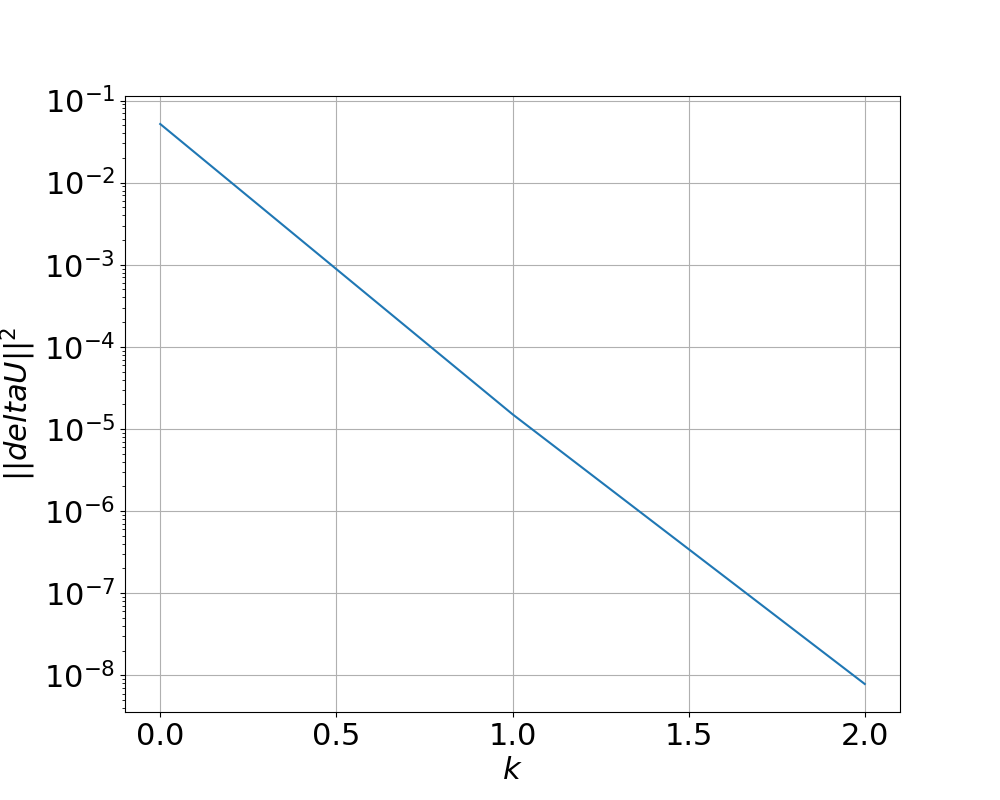
\includegraphics[width=\textwidth]{figs/Downward_Descent_smooth.png}
        \caption{Descent direction}
        \label{fig:Downward_Descent_smooth}
    \end{subfigure}
    \caption{}
\end{figure}

\section*{Python code}

The smooth reference trajectory has been defined in the python file reference\_trajectory.py. In the code several functions are defined:

\begin{itemize}
    \item \textbf{poly3(xx\_init, xx\_fin, tf, dt) }:Compute a smooth curve between xx\_init and xx\_fin connecting the two points with polynomial functions of order three. The input is computed as the gravity compensation along the obtained state reference curve. The initial and final configurations should be equilibrium points, and the reference curves are computed according to (\ref{smooth_q1}) and (\ref{smooth_q2}). The computation of $q_2$ depends on the given initial configuration. If the sum $q_1 + q_2$ at the initial configuration equals $0$, the equation for the upward arm is used. Conversely, if it equals $\pi$, the equation for the downward arm is used.  \\\\
    \textbf{Arguments}:
    \begin{itemize}
        \item xx\_init : Initial state vector in degrees.
        \item xx\_fin : Final state vector in degrees.
        \item tf : Final time in seconds.
        \item dt : Time of dicretization in seconds.
    \end{itemize}
    \textbf{Return}:
    \begin{itemize}
        \item xx\_ref : Reference curve between the two states from 0 to tf, in radiants.
        \item uu\_ref : Input reference curve.
    \end{itemize}
    
    \item \textbf{smooth\_comp(points, tf, dt) }: Compute a composition of smooth curve between state configuration points. The input is computed as the gravity compensation along the obtained state reference curve.\\\\
    \textbf{Arguments}:
    \begin{itemize}
        \item points : List of state vectors in degrees.
        \item tf : Final time in seconds.
        \item dt : Time of dicretization in second.
    \end{itemize}
    \textbf{Return}:
    \begin{itemize}
        \item xx\_ref : State reference curve in radiants.
        \item uu\_ref : Input reference curve.
    \end{itemize}

    \item \textbf{initial\_guess(xx\_ref, uu\_ref, tf, dt) }: Compute a state-input trajectory tracking the system about a smooth reference curve using an LQR solution implemented in the \textbf{LQR\_solver()} (see Task 3 for more details). \\\\
    \textbf{Arguments}:
    \begin{itemize}
        \item xx\_ref : Reference state vector.
        \item uu\_ref : Reference input vector.
        \item tf : Final time in seconds.
        \item dt : Time of dicretization in seconds.
    \end{itemize}
    \textbf{Return}:
    \begin{itemize}
        \item xx\_r : State trajectory.
        \item uu\_r : Input trajectory.
    \end{itemize}
\end{itemize}

\chapter*{Task 3}
\addcontentsline{toc}{chapter}{Task 3}

Task 3 requires linearizing the dynamics about the generated optimal trajectory $(x^{star},u^{star})$ and using the LQR algorithm to define the optimal feedback controller to track the reference trajectory.

To compute the optimal gain for the LQR regulator, we have to solve the Linear Quadratic Optimization problem stated as follows:

\begin{equation} \label{LQR}
    \begin{aligned}
        &\min_{\Delta x \Delta u} \hspace{0.1cm} \sum_{t=0}^{T-1} \Delta x_t^TQ^{reg}\Delta x_t + \Delta u_t^TR^{reg}\Delta u_t + \Delta x_T ^TQ_T^{reg}\Delta x_T \\
        &subj. to \hspace{0.5cm} \Delta x_{t+1} = A_t \Delta x_t + B_t \Delta u_t\\
        & \hspace{2cm} \Delta x_0 = 0
    \end{aligned}
\end{equation}

The cost is already a quadratic function of the displacement states and inputs with respect to the nominal trajectory.

The LQR problem can be solved using the Difference Riccati Equation, as in (\ref{Diff ricc eq}), for the matrix $P_t$ and computing the optimal gain ${K}_t^*$. 

The task assignment requires considering an initial perturbed condition different from 0. We have selected an initial perturbation of $\delta = [0.1,0.1,0,0]^T$. In addition, we have applied noise inside the control loop.

\begin{itemize}
    \item $n_a$: It is the actuation noise. It is a normally distributed random variable with mean value 0 and variance 0.01.
    \item $n_m$: It is the measurement noise. It is a normally distributed random variable with mean value 0 and variance 0.001.
\end{itemize}

The control law applies a feedforward action, which is the optimal input obtained with Newton's method, and then uses LQR to stabilize the system.

\begin{equation}
    \begin{aligned}
        &{u}_t = {K}_t^*(x_{t+1} - x_t^{star} + n_m) + u_t^{star} + n_a\\
        &{x}_{t+1} = f_d(x_t,u_t)
    \end{aligned}
\end{equation}

The weights in the regulator cost have been selected as:

\begin{equation*}
    \begin{aligned}
        &Q_t^{reg} = \begin{bmatrix}
            1000 & 0 & 0 & 0 \\
            0 & 1000 & 0 & 0 \\
            0 & 0 & 10 & 0\\
            0 & 0 & 0 & 10
        \end{bmatrix} = Q_T^{reg}\\
        &\\
    & R^{reg}_t = 10
    \end{aligned}
\end{equation*}

As we can see from the plots, the system follows the reference, and the control loop is robust with respect to noise and a perturbed initial condition.

\begin{figure}
    \centering
    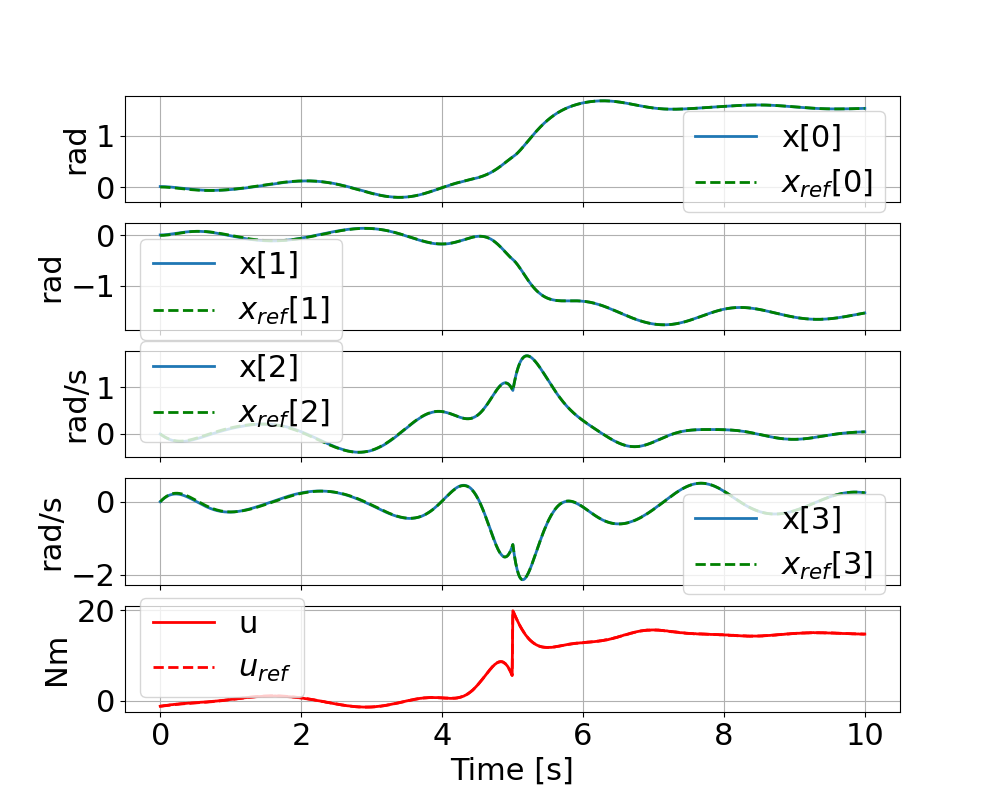
\includegraphics[width=0.8\linewidth]{figs/downward_lqr_track.png}
    \caption{Reference Tracking with LQR}
    \label{fig:downward_lqr_track}
\end{figure}

\begin{figure}
    \centering
    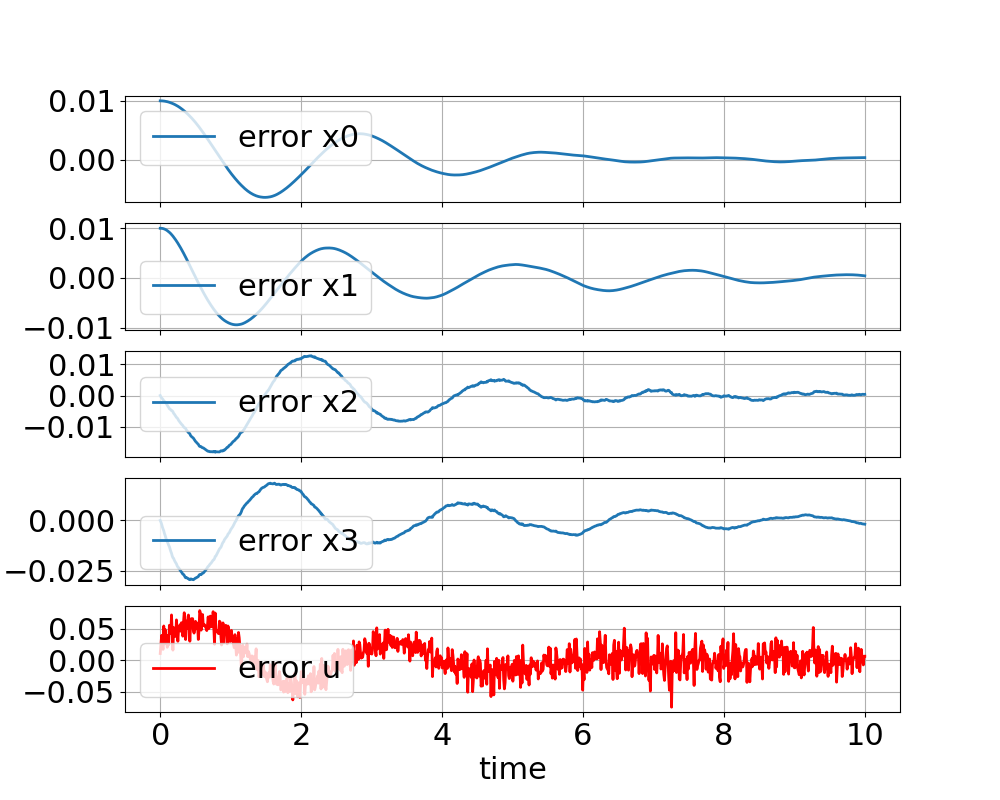
\includegraphics[width=0.8\linewidth]{figs/downward_lqr_error.png}
    \caption{Tracking error}
    \label{fig:downward_lqr_error}
\end{figure}

\begin{figure}
    \centering
    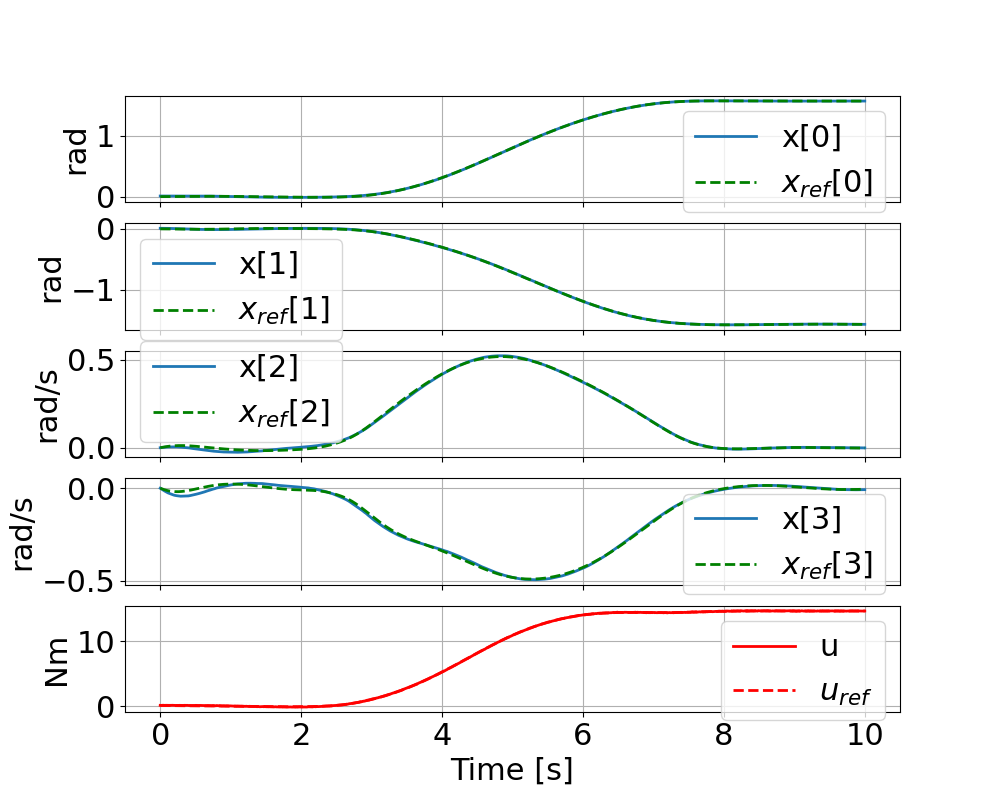
\includegraphics[width=0.8\linewidth]{figs/downward_lqr_error_smooth.png}
    \caption{Smooth reference Tracking with LQR}
    \label{fig:downward_lqr_track_smooth}
\end{figure}

\begin{figure}
    \centering
    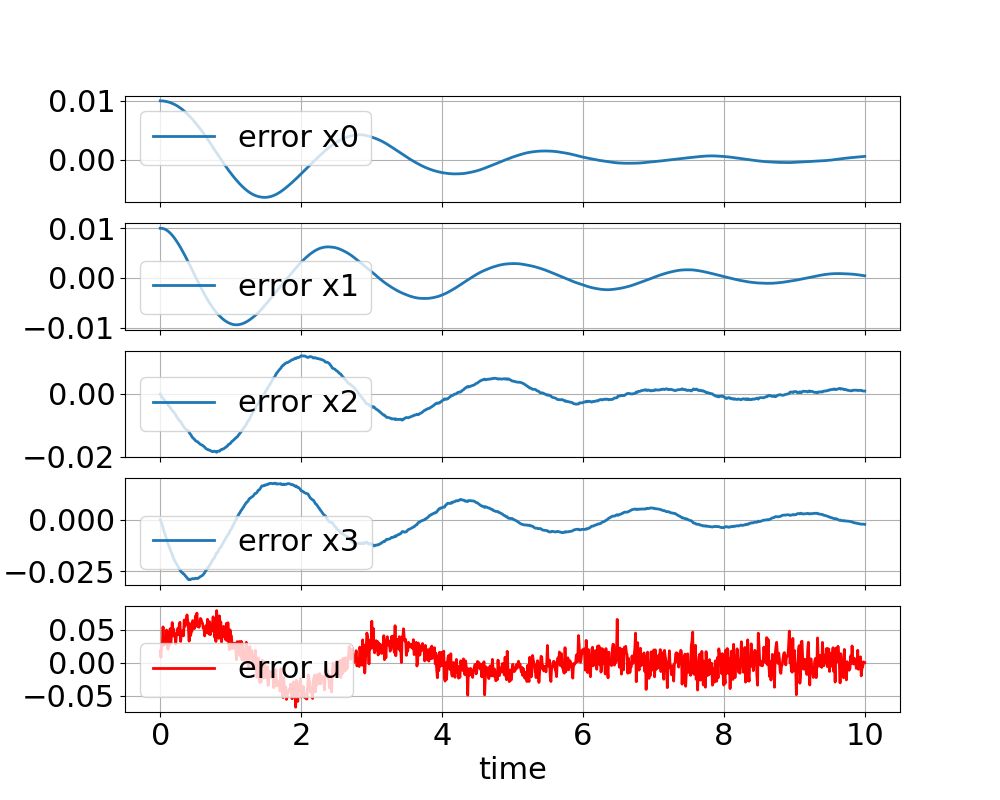
\includegraphics[width=0.8\linewidth]{figs/downward_lqr_track_smooth.png}
    \caption{Smooth reference tracking error}
    \label{fig:downward_lqr_error_smooth}
\end{figure}

\section*{Python code}

The LQR solver has been defined in the python file solver.py.

\begin{itemize}
    \item \textbf{LQR\_solver(xx\_star, uu\_star, dyn, A\_f, B\_f, QQt, RRt, tf, dt) }: Compute the optimal gain matrix $K_t^*$ for each time instant.\\\\
    \textbf{Arguments}:
    \begin{itemize}
        \item xx\_star : Optimal state reference trajectory.
        \item uu\_star : Optimal input reference trajectory.
        \item dyn : dynamic package imported from Dinamics.py.
        \item A\_f : Symbolic rappresentation of the discretized state jacobian.
        \item B\_f : Symbolic rappresentation of the discretized input jacobian.
        \item QQt : Weight matrix for the states.
        \item RRt: Weight matrix for the inputs.
        \item tf : Final simulation time, in seconds.
        \item dt : Time of dicretization in seconds.
    \end{itemize}
    \textbf{Return}:
    \begin{itemize}
        \item KK\_t : Optimal feedback gain matrix for each time instant.
    \end{itemize}
\end{itemize}

\chapter*{Task 4}
\addcontentsline{toc}{chapter}{Task 4}

Task 4 requires linearizing the dynamics about the generated optimal trajectory $(x^{star},u^{star})$ and exploiting the MPC algorithm to define a robust control law, able to track the reference trajectory.

Model Predictive Control is a technique that at each time iteration solves the whole optimal control problem for a fixed time window and applies only the first optimal input. After the first iteration, it moves the time window forward and starts computing the next optimal input. For this reason, Model Predictive Control works in an infinite time horizon.

How the optimal control problem is solved at each iteration depends on what cost and dynamics are present. This allows managing constraints directly with the certainty that they will be satisfied.

Since, in this case, constraints are not present, the cost is quadratic and the dynamics are linearized, we can solve the MPC problem by exploiting an LQR solution each time (\ref{MPC}).

The task assignment requires considering an initial perturbed condition different from 0. In addition, we have applied noise inside the control loop like in Task 3.

The control law applies a feedforward action that is the optimal input obtained with Newton's method and then uses the MPC solution to stabilize the system.

\begin{equation} \label{MPC}
    \begin{cases}
        &\\
        &\min_{\Delta x \Delta u} \hspace{0.1cm} \sum_{\tau=t}^{t+T-1} \Delta x_{\tau}^TQ^{reg}\Delta x_{\tau} + \Delta u_{\tau}^TR^{reg}\Delta u_{\tau} + \Delta x_{t+T} ^TQ_T^{reg}\Delta x_{t+T} \\
        &subj. to \hspace{0.5cm} \Delta x_{\tau+1} = A_{\tau} \Delta x_{\tau}  + B_{\tau} \Delta u_{\tau} \\
        & \hspace{2cm} \Delta x_0 =  x_t + n_m \\
        &\\
        &{u}_t = u_t^{mcp} + u_t^{star} + n_a\\
        &{x}_{t+1} = f_d(x_t,u_t)\\
        &
    \end{cases}
\end{equation}

The weights in the regulator cost have been selected as:

\begin{equation*}
    \begin{aligned}
        &Q_t^{mpc} = \begin{bmatrix}
            1000 & 0 & 0 & 0 \\
            0 & 1000 & 0 & 0 \\
            0 & 0 & 10 & 0\\
            0 & 0 & 0 & 10
        \end{bmatrix} = Q_T^{mpc}\\
        &\\
    & R^{mpc}_t = 10
    \end{aligned}
\end{equation*}

The time window we have chosen is 1 second (100 samples). We selected it by trying various values and chose a trade-off between performance and computational time.

As we can see from the plots, the system follows the reference, and the control loop is robust with respect to noise and a perturbed initial condition.

\begin{figure}
    \centering
    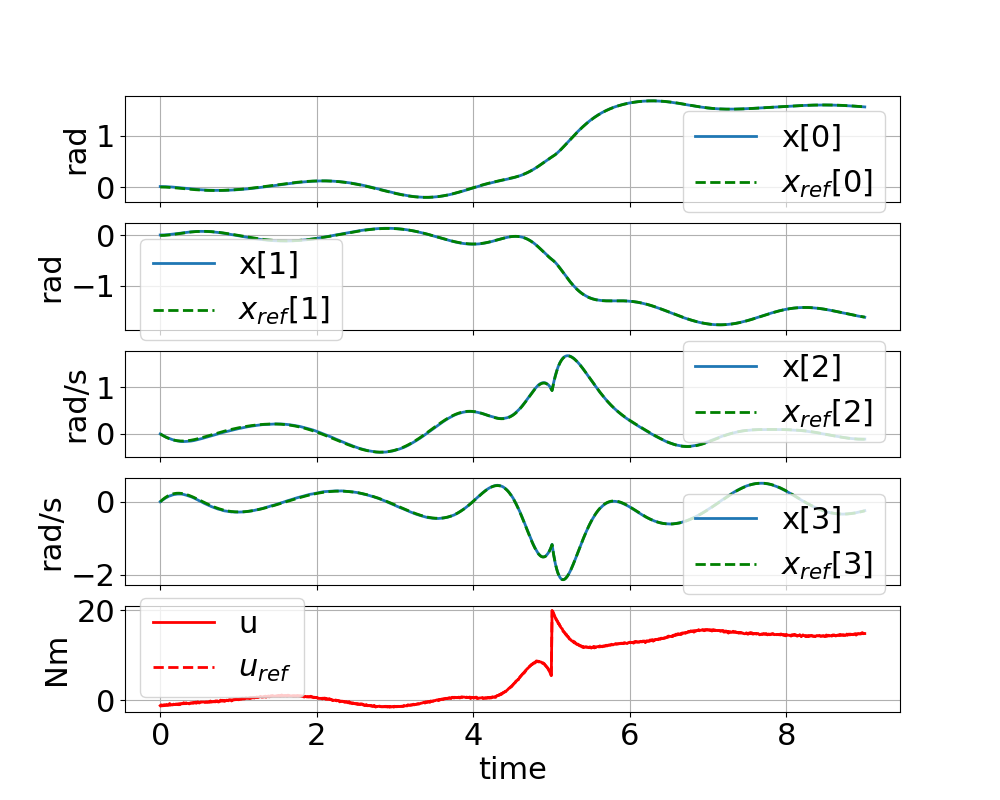
\includegraphics[width=0.8\linewidth]{figs/downward_mpc_track.png}
    \caption{Reference Tracking with MPC}
    \label{fig:downward_mpc_track}
\end{figure}

\begin{figure}
    \centering
    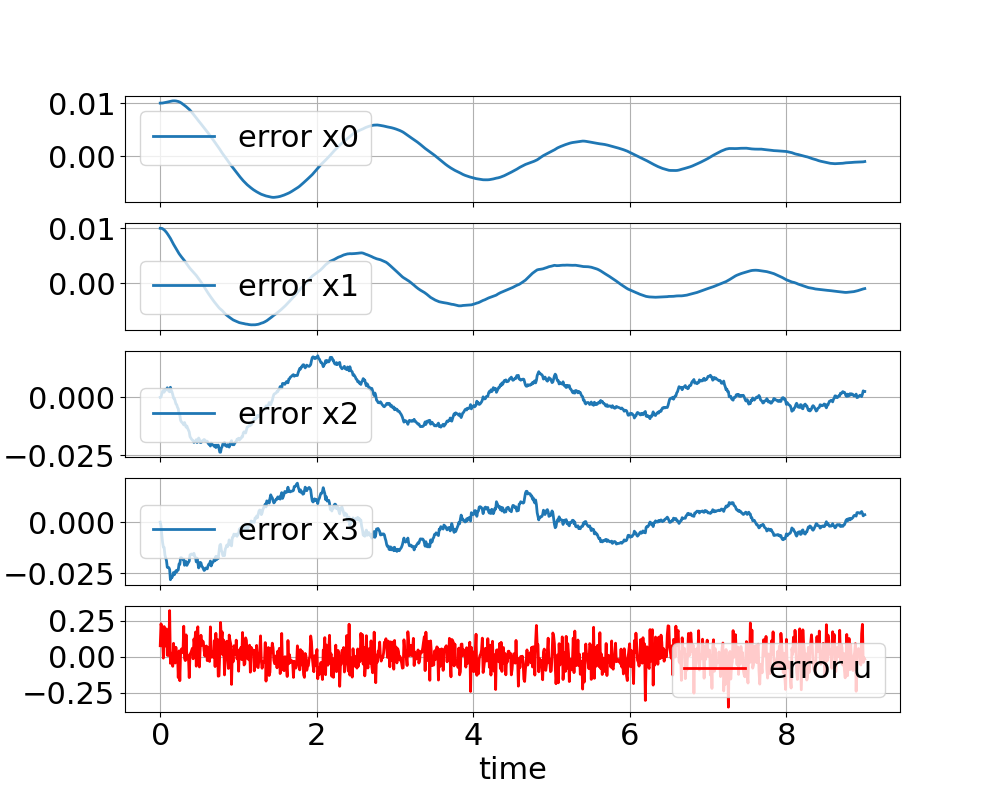
\includegraphics[width=0.8\linewidth]{figs/downward_mpc_error.png}
    \caption{Tracking error}
    \label{fig:downward_mpc_error}
\end{figure}

\begin{figure}
    \centering
    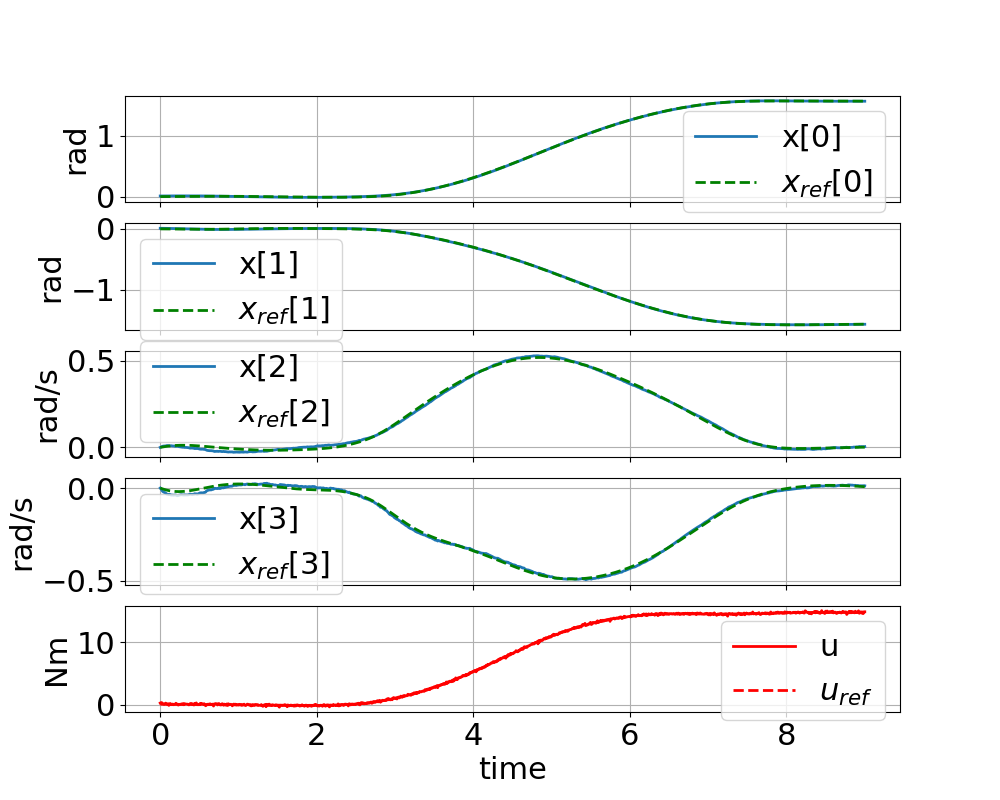
\includegraphics[width=0.8\linewidth]{figs/downward_mpc_track_smooth.png}
    \caption{Smooth reference Tracking with MPC}
    \label{fig:downward_mpc_track_smooth}
\end{figure}

\begin{figure}
    \centering
    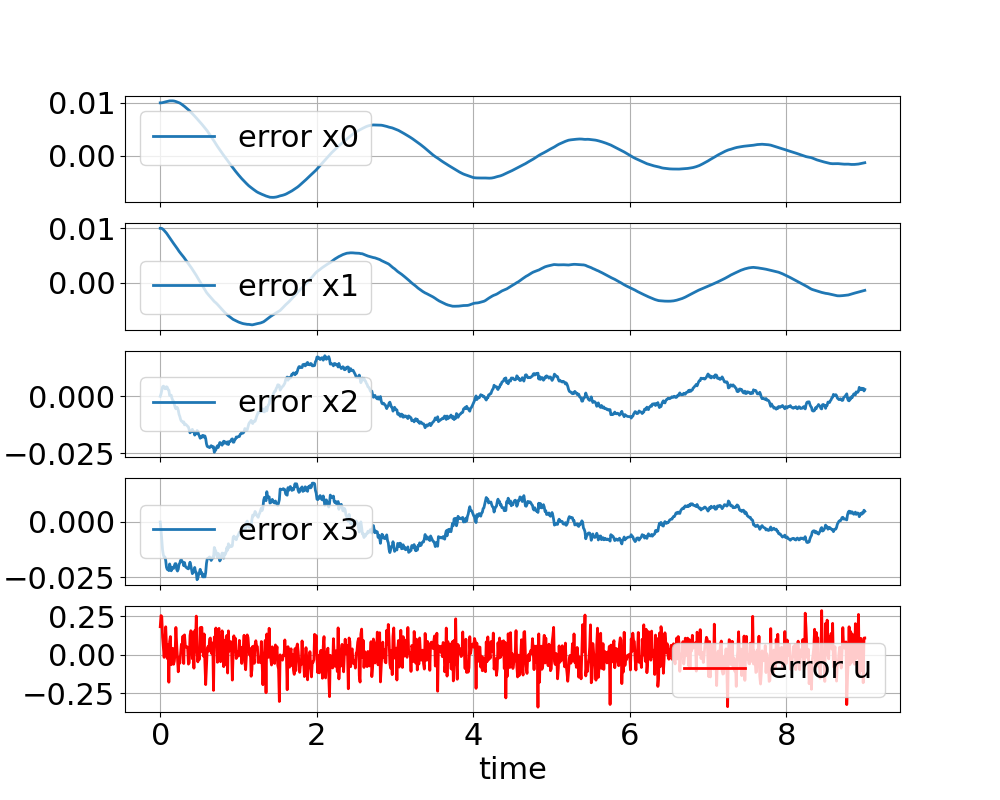
\includegraphics[width=0.8\linewidth]{figs/downward_mpc_error_smooth.png}
    \caption{Smooth reference tracking error}
    \label{fig:downward_mpc_error_smooth}
\end{figure}

\section*{Python code}
The MPC solver is defined in the Python file \texttt{solver.py}. The function calls the LQR function to obtain a gain \( K^* \), and then uses it to compute the optimal input as \( \Delta u_t = K_t \cdot \Delta x_t \).

\begin{itemize}
    \item \textbf{solver\_linear\_mpc(dyn, A\_f, B\_f, QQ, RR, QQf, xx\_t, xx\_star, uu\_star, dt, T\_pred = 20) }: Compute the optimal gain matrix $K_t^*$ for each time instant.\\\\
    \textbf{Arguments}:
    \begin{itemize}
        \item dyn : dynamic package imported from Dinamics.py.
        \item A\_f : Symbolic rappresentation of the discretized state jacobian.
        \item B\_f : Symbolic rappresentation of the discretized input jacobian.
        \item QQ : Weight matrix for the states.
        \item RR: Weight matrix for the inputs.
        \item QQf : Weight matrix for the states at the final time T.
        \item xx\_t : measured input at time t.
        \item xx\_star : Optimal state reference trajectory in the time window.
        \item uu\_star : Optimal input reference trajectory in the time window.
        \item dt : Time of dicretization in seconds.
        \item T\_pred : Time prediction window size in seconds.
    \end{itemize}
    \textbf{Return}:
    \begin{itemize}
        \item uu\_mpc: Optimal input at time t.
    \end{itemize}
\end{itemize}

\chapter*{Animation}
\addcontentsline{toc}{chapter}{Animation}

For the animation, the subpackage \texttt{matplotlib.animation} has been used. The \texttt{FuncAnimation} function allows displaying consecutive plots as an animation. The robot is presented as a chain of two segments with dots at the extremities. The reference trajectory for the end-effector is plotted as a dashed line, allowing the motion to be appreciated from the beginning.

\begin{figure}[H]
    \centering
    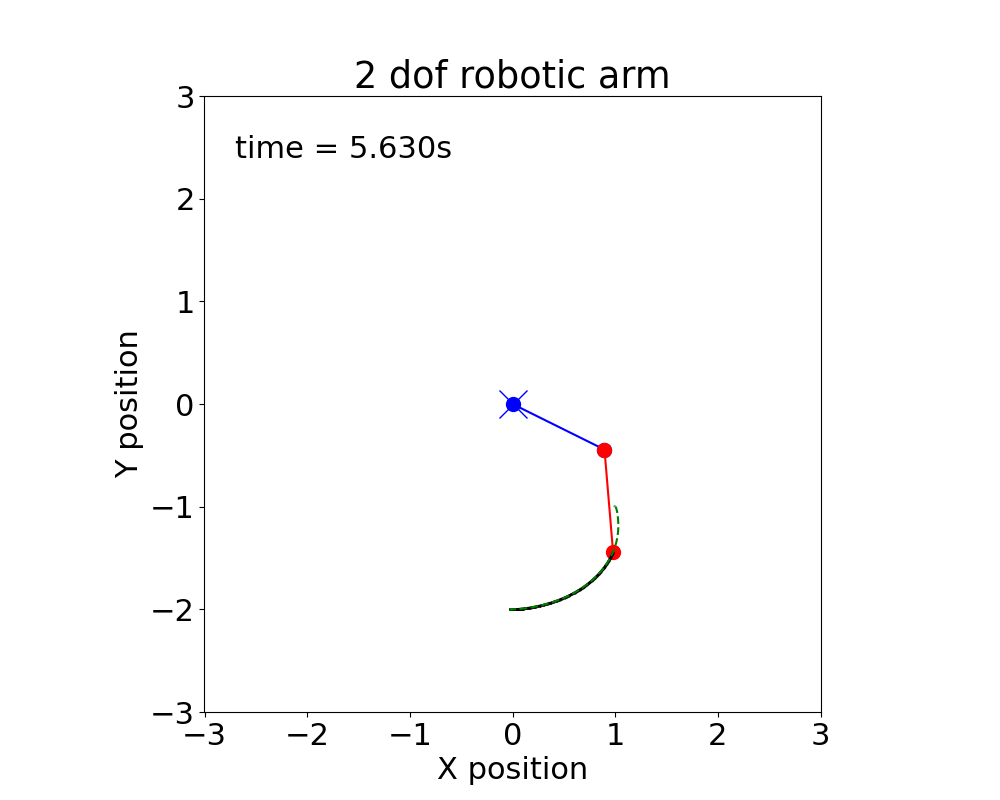
\includegraphics[width=0.8\linewidth]{figs/downward_video_0.png}
    \caption{Animation for the smooth trajectory of Task 2}
    \label{fig:downward_video_0}
\end{figure}


For the purpose of showing the various steps of the project, a simple trajectory has been presented in the previous figures. However, we have tested different trajectories that will be presented below with some plots and animations.

\subsection*{Swing up}

\begin{figure}[H]
    \centering
    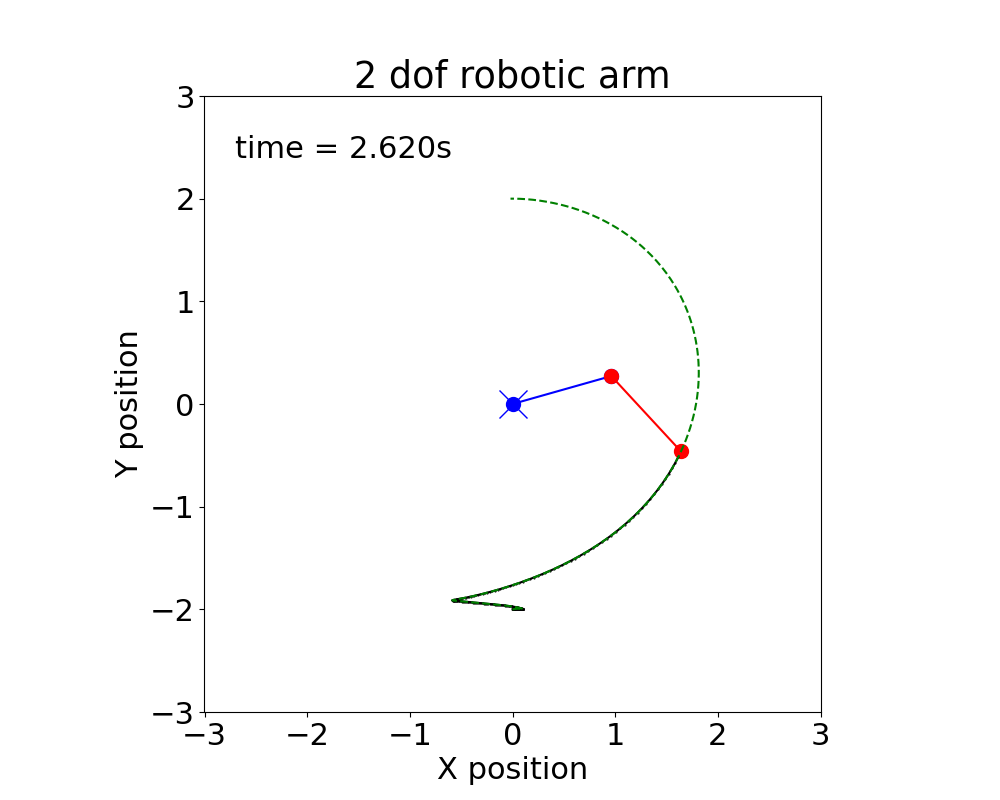
\includegraphics[width=0.8\linewidth]{figs/swing_video.png}
    \caption{Animation for the swing up trajectory}
    \label{fig:swing_video}
\end{figure}

\begin{figure}[H]
    \centering
    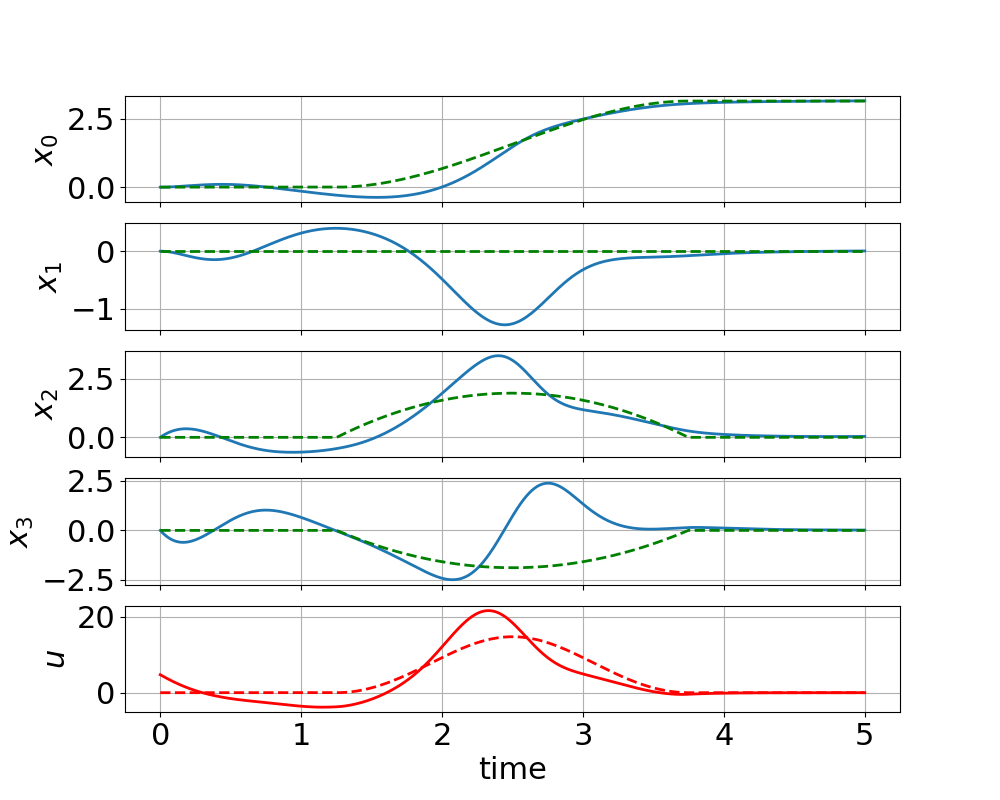
\includegraphics[width=0.8\linewidth]{figs/swing_result.png}
    \caption{Swing up final result}
    \label{fig:swing_result}
\end{figure}

\subsection*{Circular motion}

\begin{figure}[H]
    \centering
    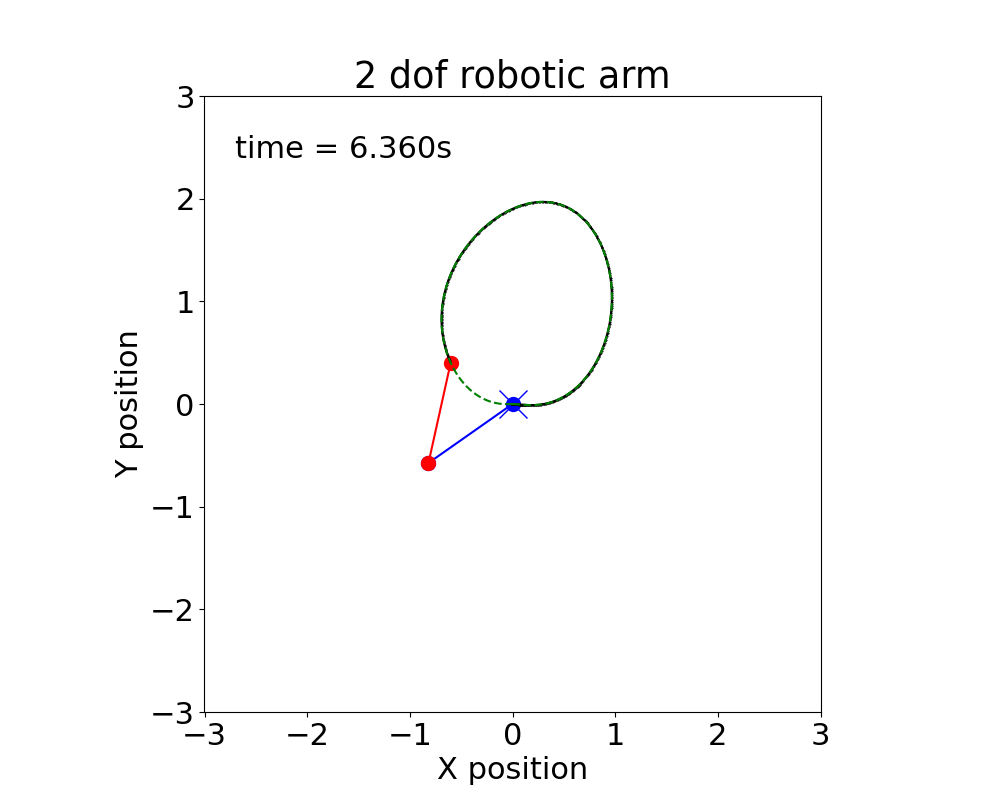
\includegraphics[width=0.8\linewidth]{figs/circle_video.png}
    \caption{Animation for the circular trajectory}
    \label{fig:swing_video}
\end{figure}

\begin{figure}[H]
    \centering
    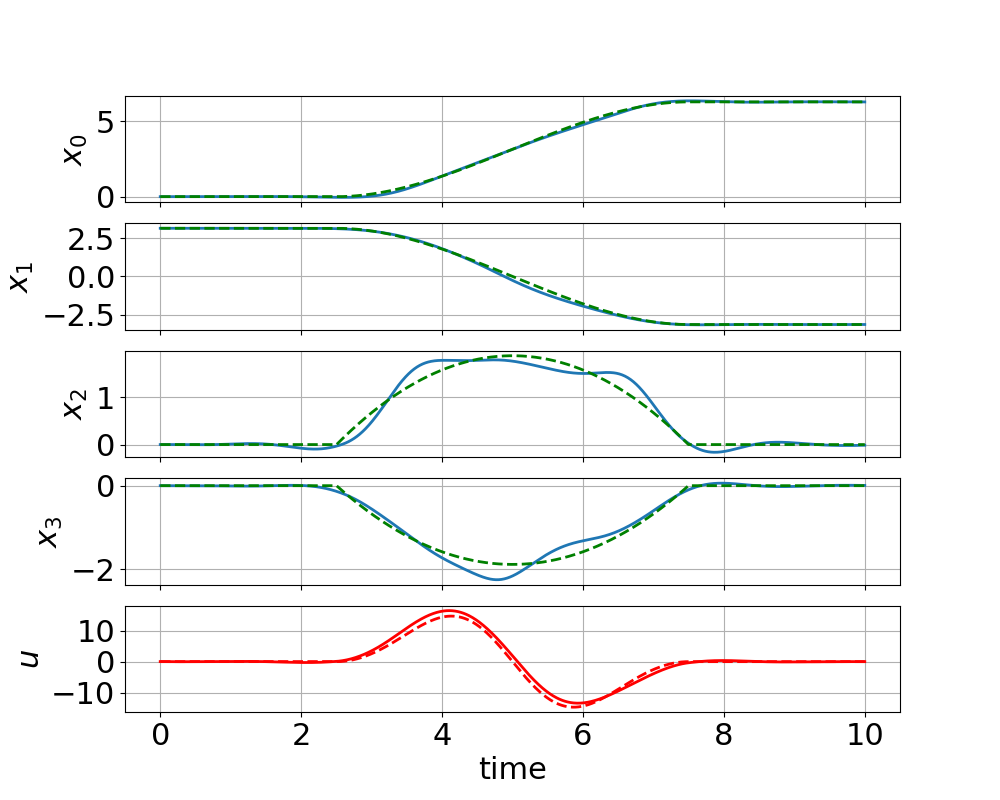
\includegraphics[width=0.8\linewidth]{figs/circle_result.png}
    \caption{Circular motion final result}
    \label{fig:circle_result}
\end{figure}

%%%%%%%%%% Conclusions %%%%%%%%%%
\chapter*{Conclusions}
\addcontentsline{toc}{chapter}{Conclusions} 

The project showed how the Optimal Control framework can effectively manage complex systems. It successfully controlled the underactuated manipulator and dealt with time-varying linear systems, such as the linearized model of the manipulator. Additionally, the framework demonstrated its capability to generate optimal trajectories for the system, ensuring smooth and efficient movement while satisfying the system's constraints.

The results proved that the control methods are robust, even when there is noise, making them reliable for practical use. Additionally, the exploration of different approaches highlighted the flexibility of the Optimal Control framework in solving similar problems.

%%%%%%%%%% Bibliography %%%%%%%%%%%
\bibliography{bibliography}{}
\bibliographystyle{plain}
\addcontentsline{toc}{chapter}{Bibliography}
\nocite{*}
%%%%%%%%%%%%%%%%%%%%%%%%%%%%%%%%%%%%%%

\end{document}


\begin{equation*}
    \mathcal{X}_{\text{eq}} = \{x \in \mathcal{X} \mid {x = [x_1, x_2, 0, 0] \land u = G_1(x)} ;\hspace{0.1cm} x_1 \in \mathrm{}{R}, x_2 \in \mathrm{}{R}, x_1 + x_2 = {0 \lor \pi} \}
\end{equation*}